%!TEX program = xelatex
%\documentclass[cn,hazy,blue,14pt,screen]{elegantnote}

\documentclass[cn,
               %mode=geye,
               mode=hazy,
               color=blue,
               %color=green,
               %color=cyan,
               %color=sakura,
               11pt,
               %device=pc,      % double pages for pc
               device=normal,  % a4 normal page
               %device=screen  % 4:3 PPT size
               ]{elegantnote}

\usepackage{amsmath,amsbsy,amssymb,amsfonts}
\usepackage{bm}
\usepackage{extarrows}
\usepackage{diagbox}

\usepackage{listings}
%\usepackage[framed,numbered,autolinebreaks,useliterate]{mcode}

%\usepackage[numbered,autolinebreaks,useliterate]{mcode}
\usepackage[numbered,framed]{matlab-prettifier}

\iffalse
\definecolor{mygreen}{rgb}{1 1 0.87}
\definecolor{mygray}{rgb}{0.0,1.,1.}
\definecolor{mymauve}{rgb}{0.58,0,0.82}
\lstset{
backgroundcolor=\color{mygreen},   % choose the background color,
flexiblecolumns=true, %
breaklines=true, %对过长的代码自动换行
breakautoindent=true,%
escapeinside=``,
language=Matlab,
}
\fi


%\newtheorem{solution*}{解} %
\newtheorem*{solution}{解.}

\definecolor{myred}{rgb}{0.84, 0.04, 0.33}

\def
\theequation{\thesection.\arabic{equation}}
\numberwithin{equation}{section}
\newcommand*{\abs}[1]{\lvert#1\rvert}
\newcommand*{\Abs}[1]{\big\lvert#1\big\rvert}
\newcommand*{\ABS}[1]{\Big\lvert#1\Big\rvert}
%\newcommand*{\norm}[1]{\left\lVert #1 \right\rVert}
\newcommand*{\norm}[1]{\lVert #1 \rVert}
\newcommand*{\Norm}[1]{\big\lVert #1 \big\rVert}
\newcommand*{\NOrm}[1]{\Big\lVert #1 \Big\rVert}
\newcommand*{\NORM}[1]{\left\lVert #1 \right\rVert}
\newcommand*{\tnorm}[1]{\interleave#1\interleave}
\newcommand*{\jump}[1]{\llbracket #1\rrbracket}
%\newcommand*{\jump}[1]{\lBrack #1\rBrack}
\newcommand*{\Jump}[1]{\left\llbracket #1\right\rrbracket}
\newcommand*{\JUMP}[1]{\Big\llBracket #1 \Big\rrBracket}
\def\sech{\mathrm{sech}}
\def\mathi{\mathrm{i}}
\def\tr{\mathrm{tr}}
\def\mathe{\mathrm{e}}
%\newcommand\mathd{\mathrm{d}}
\newcommand\mathd{\,d}
\newcommand\bsm{\boldsymbol}
%\def\mathds{\mathrm{~d}}
%\def\mathdx{\mathrm{~d\bf{x}}}
\def\mathds{\,ds}
%\def\mathd{\,d}
\def\mathdx{\,d{\bm x}}
\def\mathdy{\,d{\bm y}}
\renewcommand{\Re}{\operatorname{Re}}
\renewcommand{\Im}{\operatorname{Im}}




\title{数值分析原理课后习题}

\author{李琦 \\ Email: liqihao2000@126.com
        %\and
        }

\institute{信息与计算科学系\\长安大学理学院}

%\version{1.00}
\date{\zhtoday}

\usepackage{array}

\begin{document}

\maketitle

\vspace{30mm}

\centerline{
教材: 数值分析原理. 封建湖, 车刚明, 聂玉峰 编著. 北京: 科学出版社, 2001.9
}

\iffalse
\centerline{
  
\includegraphics[width=0.2\textwidth]{logo-blue.png}
}
\fi

\newpage

\section*{习题 1}

\begin{enumerate}
  \item 请指出如下有效数的绝对误差限、相对误差限和有效数字位数:\\
        \centerline{
        $49\times 10^{-2}$,\quad $0.0490,$\quad $490.00.$
        }
        \begin{solution}
        \begin{enumerate}
          \item 记 $x_1=49\times 10^{-2}=0.49\times 10^{0},$ $m=0,$ $n=p=2,$ $2$位有效数字.\\[2mm]
            $\abs{x_1}\leq\varepsilon=\dfrac{1}{2}\times10^{m-n}=\frac{1}{2}\times10^{-2}=0.005.$\\[3mm]
            $\varepsilon_r=\dfrac{\varepsilon}{x_1}=\dfrac{0.005}{0.49}\approx0.0102.$
          \item 记 $x_2=0.0490=0.490\times 10^{-1},$ $m=-1,$ $n=p=3,$ $3$位有效数字.\\[2mm]
            $\abs{x_2}\leq\varepsilon=\dfrac{1}{2}\times10^{m-n}=\frac{1}{2}\times10^{-4}=0.00005.$\\[3mm]
            $\varepsilon_r=\dfrac{\varepsilon}{x_2}=\dfrac{0.005}{0.0490}\approx0.00102.$
          \item 记 $x_3=490.00=0.49000\times 10^{3},$ $m=3,$ $n=p=5,$ $5$位有效数字.\\[2mm]
            $\abs{x_3}\leq\varepsilon=\dfrac{1}{2}\times10^{m-n}=\frac{1}{2}\times10^{-2}=0.005.$\\[3mm]
            $\varepsilon_r=\dfrac{\varepsilon}{x_3}=\dfrac{0.005}{490.00}\approx0.0000102.$
        \end{enumerate}
        \end{solution}

  \item 将22/7作为 $\pi$ 的近似值, 它有几位有效数字, 绝对误差限和相对误差限各为多少?
        \begin{solution}
        $\pi=0.314159265\dots\times10^{1},$ $22/7\approx0.31428571428\times10^{1},$ $m=1,$ $n=3.$\\
        $\Abs{\frac{22}{7}-\pi}\approx 0.1264489\times10^{-2}=0.126\times10^{1-3}\leq \frac{1}{2}\times10^{1-3},$ 故有效数字为 $3$ 位. $\varepsilon=0.0013,$ $\varepsilon_r=0.0013/(22/7)=0.00041.$
        \end{solution}

  \item 要使 $\sqrt{101}$ 的相对误差不超过 $\frac{1}{2}\times 10^{-4},$ 至少需要保留多少位有效数字.
      \begin{solution}
      $\sqrt{101}\approx 10.05=0.1005\times10^{2},$ 故标准形式中 $x_1=1.$ 根据书中第6页定理 1.1 知,
      $$ \abs{e^{*}_r}\leq \dfrac{1}{2x_1}\times10^{1-n}=\dfrac{1}{2}\times10^{1-n}\leq \dfrac{1}{2}\times10^{-4}.$$ 由上式得 $n\geq 5.$ 因此, 至少需要保留 $5$ 位有效数字.
      \end{solution}

  \item 设 $x^*$ 为 $x$ 的近似数, 证明 $\sqrt[n]{x^*}$ 的相对误差大约为 $x^*$ 相对误差的 $\frac{1}{n}$ 倍.
      \begin{proof}
       设 $y=f(x)=\sqrt[n]{x},$ 则有 $f'(x)=\frac{1}{n}x^{
       \frac{1}{n}-1}.$ 记 $y^*=\sqrt[n]{x^*},$ 那么相对误差
       $$ e_r(y^*)=\dfrac{y^*-y}{y^*}=\dfrac{\sqrt[n]{x^*}-\sqrt[n]{x}}{\sqrt[n]{x^*}}=\dfrac{f'(x^*)(x^*-x)}{{x^*}^{\frac{1}{n}}}=\dfrac{1}{n}e_r(x^*).$$
       \\证毕.
      \end{proof}

  \item 某矩形的长和宽大约为 100cm 和 50cm, 应该选用最小刻度为多少 cm 的测量工具, 才能保证计算出的面积误差不超过 0.15cm$^2.$
      \begin{solution}
      面积的误差限为 $\varepsilon(x_1x_2).$ 由书中第8页公式(1.9)知
      \begin{align*}
      \varepsilon(x_1^*x_2^*)&\approx\abs{x_1^*}\varepsilon(x_1^*)+\abs{x_2}\varepsilon(x_1^*)\\
      &=50\varepsilon(x_1^*)+150\varepsilon(x_1^*)\\
      &\leq 150\max\{\varepsilon(x_1^*),\varepsilon(x_2^*)\}
      \end{align*}
      由题意要使 $150\max\{\varepsilon(x_1^*),\varepsilon(x_2^*)\}\leq 0.015.$ 得 $\max\{\varepsilon(x_1^*),\varepsilon(x_2^*)\}\leq 0.001.$ 所以, 应该选用最小刻度为 $0.001$ cm 的测量工具.
      \end{solution}

  \item 设 $x=5\pm 0.1,$ $y=5\pm 0.1,$ 试估计出 $a=y/(x+1)$ 的取值范围.
      \begin{solution}
      $x\in[5-0.1,5+0.1],$ $y\in[5-0.1, 5+0.1].$ 所以 $x\in[6-0.1,6+0.1],$ 进一步 $1/x\in[1/(6+0.1),1/(6-0.1)].$
      因此
      \begin{align*}
      a&=y/(x+1)=[5-0.1,5+0.1]*[1/(6+0.1),1/(6-0.1)]\\
       &=[4.9/6.1, 5.1/5.9]\approx[0.803278, 0.864407].
      \end{align*}
      \end{solution}


  \item 论证当 $x^*$ 是 $x$ 的较好近似时, 函数值的绝对误差、自变量的相对误差、相对误差意义下的条件数之间满足如下近似公式
      $$ \varepsilon_r(f^*)\approx \mathrm{cond}_r(f(x^*))\varepsilon_r(x^*).$$
      \begin{proof}
       $\text{左边}=\varepsilon_r(f^*)=\dfrac{f(x^*)-f(x)}{f(x^*)}=\dfrac{f'(x^*-\theta(x^*-x))(x^*-x)}{f(x^*)},$\\
       $\text{右边}=\mathrm{cond}_r(f(x^*))\varepsilon_r(x^*)=x^*\dfrac{f'(x^*)}{f(x^*)}\dfrac{x^*-1}{x^*}=\dfrac{f'(x)(x^*-x)}{f(x^*)}.$\\
       又因为 $x^*$ 是 $x$ 的较好近似, 所以 $f'(x^*-\theta(x^*-x))\approx f'(x^*),$ 即得到结论.
      \end{proof}
      \begin{note}
      \color{myred}
      最后的结论是左边$\approx$右边, 但是很多同学证明出来的结果是 $=$ 而不是 $\approx.$
      \end{note}

  \item 计算函数 $y=\sin(n^3x)$ 在 $x=0.0001$ 附近的函数值, 当 $n=100$ 时, 试估计满足函数值相对误差不超过 $0.1\%$ 时的自变量相对误差限和绝对误差限.
      \begin{solution}
      记$f'(x)=y'=n^3\cos(n^3x).$ 相对误差
      \begin{align*}
      e_r(y^*)=\dfrac{x^*}{f(x^*)}f'(x^*)e_r(x^*)=\dfrac{x^*n^3\cos(n^3x^*)}{\sin(n^3x^*)}e_r(x^*).
      \end{align*}
      当 $n=100,$ $x=0.0001$ 时, 函数值相对误差不超过 $0.1\%,$ 即
      $$\dfrac{100}{\tan(100)}e_r(x^*)\leq 0.001,$$
      得 $e_r(x^*)\leq 0.5872\times10^{-5},$ 绝对误差 $e(x^*)=x^*e_r(x^*)=0.5872\times10^{-9}.$
      \end{solution}
      \begin{note}
      \color{myred}
      很多同学用手机计算器计算出 $\tan(100)\approx-5.671,$ 如果是这样情况的话, 同学们再计算一下是否有 $\tan(45)=1,$ 如果是的话, 那么你用的计算输入参数的单位是$^\circ$ 而不是弧度. 这个习题需要用孤独计算.
      \end{note}

  \item 对于 32 位单精度实数系统, 使用迭代格式算法
        $$x_0=4, x_{n+1}=x_n^2, n=1,2,3,\cdots$$
        迭代多少次将产生上溢.
        \begin{solution}
        $x_1=x_0^2,$ $x_2=x_1^2=x_0^4,$ $x_3=x_2^2=x_0^8,$ $\cdots,$ $x_n=x_{n-1}^2=x_{n-k}^{2^k}=x_0^{2^n},$
        使得在 32 位单精度实数系统不上溢, 那么 $x_n=x_0^{2^n}=4^{2^n}\leq 2^{2^7-1},$ 即 $2\cdot2^n=2^{n+1}\leq 2^7-1,$ 得到 $n = \frac{\lg(127)}{\lg(2)}-1\approx5.989\leq 6.$ 因此, 该格式迭代 6 次将产生上溢.
        \end{solution}

  \item 请设计求解方程 $x^2+2px+q=0$ 根的一个有效算法, 要求它也能够适用于 $p\gg\abs{q}$ 时的情形. 用所设计算法以及求根公式计算 $p=240.05,$ $q=1.00$ 时方程根的近似值(计算过程保留2位小数), 并给出两个根近似值的相对误差界.
      \begin{solution}
      求根公式 $x=-p\pm\sqrt{p^2-q}.$ 当 $p\gg\abs{q}$ 时, $-p$ 和 $\sqrt{p^2-q}$ 是两个相近的数, 为避免相近的数相减, 取求根公式.
      $x_1=-p-\sqrt{p^2-q},$ $x_2=\dfrac{q}{x_1}.$\\
      $\sqrt{p^2-q}=\sqrt{(240.05)^2-1}\approx0.24\times10^3.$ 得 $x_1\approx -480=-0.48\times10^3,$ $x_2\approx -0.21\times10^{-2}.$ \\
      $\varepsilon(x_1)=\frac{1}{2}\times10^{m-n}=\frac{1}{2}\times10^{3-2}=5,$ \\ $\varepsilon(x_2)=\frac{1}{2}\times10^{m-n}=\frac{1}{2}\times10^{-2-2}=0.00005,$
      \end{solution}

  \item 设有 64 位浮点系统: 尾数符号位占1位, 尾数数值占52位, 阶码符号位占1位, 阶码数值占10位. 请推算在此系统下实数的浮点表示能够有多少位有效数字, 并计算该浮点系统的上溢界和下溢界.
      \begin{solution}
      类似于本书第 12 页, 有
      $$\abs{e_r^*}=\ABS{\dfrac{fl(x)-x}{fl(x)}}\leq \dfrac{2^{p-1-52}}{2^{p-1}}=2^{-52}=10^n,$$
      得 $n=\lg(2^{-52})\approx-15.65.$ 因此双精度系统下实数的浮点表示能够有 15$\sim$16 位有效数字.\\
      上溢界: $2^{2^{10-1}}=10^m,$ 得 $m=\lg(2^{2^{10-1}})\approx307.95,$\\
      下溢界: $2^{2^{-10}}=10^m,$ 得 $m=\lg(2^{2^{-10}})\approx-308.25.$
      \end{solution}


\end{enumerate}

\newpage

\section*{习题 2}

\begin{enumerate}
  \item 对于下面给出的函数值表, 试构造合适的二次 Lagrange 插值多项式计算 $f(1.8)$ 的近似值.
      \begin{center}
        \begin{tabular}{c|c|c|c|c|c}
            \toprule
            $x$   & -1   &  0   &   1  &   2  & 3    \\
            \midrule
            $f(x)$& 1.21 & 1.42 & 1.72 & 1.67 & 1.58 \\
            \bottomrule
        \end{tabular}
      \end{center}
  \begin{solution}
  根据误差估计式, 选 $x_0=1,$ $x_1=2,$ $x_2=3$ 为插值节点, Lagrange 插值基函数为
  \begin{align*}
    & l_0(x)=\dfrac{(x-x_1)(x-x_2)}{(x_0-x_1)(x_0-x_2)}=\dfrac{(x-2)(x-3)}{(1-2)(1-3)}=\dfrac{1}{2} (x-2)(x-3),\\
    & l_1(x)=\dfrac{(x-x_0)(x-x_2)}{(x_1-x_0)(x_1-x_2)}=\dfrac{(x-1)(x-3)}{(2-1)(2-3)}=- (x-1)(x-3), \\
    & l_2(x)=\dfrac{(x-x_0)(x-x_1)}{(x_2-x_0)(x_2-x_1)}=\dfrac{(x-1)(x-2)}{(3-1)(3-2)}=\dfrac{1}{2} (x-1)(x-2).
  \end{align*}
  二次多项式为
  \begin{align*}
  L_2(x) & = f(x_0)l_0(x)+f(x_1)l_1(x)+f(x_2)l_2(x)\\
         & = 1.72\dfrac{(x-2)(x-3)}{2} - 1.67(x-1)(x-3)+1.58\dfrac{(x-1)(x-2)}{2},
  \end{align*}
  于是
   $$ f(1.8)\approx L_2(1.8)=1.6832.$$
  \end{solution}

  \item 已知 $f(x)=\sin x$ 的如下函数值表,
    \begin{center}
        \begin{tabular}{c|c|c|c}
            \toprule
            $x$   & 1.0   &  1.5   &   2.0 \\
            \midrule
            $\sin x$& 0.8415 & 0.9975 & 0.9093 \\
            \bottomrule
        \end{tabular}
      \end{center}
      试用二次插值多项式计算 $\sin(1.8)$ 的近似值 $L_2(1.8),$ 并用插值余项估计其误差限 $\varepsilon,$ $\varepsilon$ 与 $\Abs{\sin(1.8) - L_2(1.8)}$ 相差大吗? 试解释其原因. 对任意 $x\in [1,2]$ 估计用 $L_2(x)$ 近似 $\sin x$ 的插值误差限.
    \begin{solution}
    以 $x_0=1.0,$ $x_1=1.5,$ $x_2=2.0$ 为插值节点, Lagrange 插值基函数为
      \begin{align*}
        & l_0(x)=\dfrac{(x-x_1)(x-x_2)}{(x_0-x_1)(x_0-x_2)}=\dfrac{(x-1.5)(x-2)}{(1-1.5)(1-2)}=2 (x-1.5)(x-2),\\
        & l_1(x)=\dfrac{(x-x_0)(x-x_2)}{(x_1-x_0)(x_1-x_2)}=\dfrac{(x-1)(x-2)}{(1.5-1)(1.5-2)}=-4 (x-1)(x-2), \\
        & l_2(x)=\dfrac{(x-x_0)(x-x_1)}{(x_2-x_0)(x_2-x_1)}=\dfrac{(x-1)(x-1.5)}{(2-1)(2-1.5)}=2 (x-1)(x-1.5).
      \end{align*}
  二次多项式为
  \begin{align*}
  L_2(x) & = f(x_0)l_0(x)+f(x_1)l_1(x)+f(x_2)l_2(x),
  \end{align*}
  于是
   \begin{align*}
   \sin(1.8)\approx L_2(1.8)&=0.8415l_0(1.8)+0.9975l_1(1.8)+0.9093l_2(1.8)\\
   &=0.973884.
   \end{align*}
   插值余项
   $$ R_2(x)=f(x)-L_2(x)=\dfrac{f'''(\zeta)}{3!}\omega_3(x)\leq \dfrac{1}{6}(x-x_0)(x-x_1)(x-x_2),$$
   所以误差限为 $$\varepsilon=\dfrac{1}{6}(1.8-1)(1.8-1.5)(1.8-2)=0.008,$$
   误差为
   $$\abs{\sin(1.8)-L_2(1.8)}\approx 0.00003637,$$
   这与 $\varepsilon$ 相差较大, 这是因为 $\varepsilon$ 中导数的绝对值估计偏大. 插值误差限为
   $$ \varepsilon=\max\limits_{x\in[1,2]}\abs{R_2(x)}=\max\limits_{x\in[1,2]}\ABS{\dfrac{1}{6}(x-x_0)(x-x_1)(x-x_2)}=0.00802.$$
    \end{solution}


  \item 取节点 $x_0=0,$ $x_1=1$ 对函数 $y=\mathe^{-x}$ 作线性插值, 用该插值函数计算 $e^{-0.5}$ 和 $e^{-1.5}$ 的近似值, 并比较这两个近似值的误差限, 比较结果对你有什么启示.
      \begin{solution}
      对插值数据 $x_0=0,$ $x_1=1,$ $f(x_0)=1,$ $f(x_1)=e^{-1}$ 做线性插值,
      $$ L_1(x) = 1\dfrac{(x-1)}{0-1}+e^{-1}\dfrac{x-0}{1-0}=(e^{-1}-1)x+1,$$
      所以 $L_1(0.5)\approx 0.6839,$ $L_1(1.5)\approx 0.0518,$
      误差限
      $$\varepsilon(0.5)=\abs{e^{-0.5}-L_1(0.5)}=0.0774, $$
      $$\varepsilon(1.5)=\abs{e^{-1.5}-L_1(1.5)}=0.1713, $$
      由上面的计算结果可以看出内插法要好于外插法.
      \end{solution}

  \item 已知如下的函数表:
      \begin{center}
        \begin{tabular}{c|c|c|c|c}
            \toprule
            $x$   & 0.1  &  0.2   &   0.3  &   0.4  \\
            \midrule
            $f(x)$& -2 & 0 & 1 & 2  \\
            \bottomrule
        \end{tabular}
      \end{center}
      使用反插值法求解方程 $f(x)=0.5$ 在区间 $[0.1, 0.4]$ 内根的近似值.
      \begin{solution}
      对于 $y=f(x)$ 的反函数 $x=f^{-1}(y)$ 进行三次插值, 插值函数为
      \begin{align*}
      L_3(y) &= f^{-1}(y_0)\dfrac{(y-y_1)(y-y_2)(y-y_3)}{(y_0-y_1)(y_0-y_2)(y_0-y_3)}\\
      &\quad+ f^{-1}(y_1)\dfrac{(y-y_0)(y-y_2)(y-y_3)}{(y_1-y_0)(y_1-y_2)(y_1-y_3)}\\
      &\quad+ f^{-1}(y_2)\dfrac{(y-y_0)(y-y_1)(y-y_3)}{(y_2-y_0)(y_2-y_1)(y_2-y_3)}\\
      &\quad+ f^{-1}(y_3)\dfrac{(y-y_0)(y-y_1)(y-y_2)}{(y_3-y_0)(y_3-y_1)(y_3-y_2)}\\
      &=0.1\dfrac{x(x-1)(x-2)}{-24}+0.2\dfrac{(x^2-4)(x-1)}{4}\\
      &\quad +0.3\dfrac{x(x^2-4)}{-3}+0.4\dfrac{(x+2)x(x-1)}{8},
      \end{align*}
      于是有
          $$ x^*\approx L_3(0.5)=0.2484375.$$
      \end{solution}

  \item 证明关于互异节点 $\{x_i\}_{i=0}^n$ 的 Lagrange 插值基函数 $\{l_i(x)\}_{i=0}^n$ 满足恒等式 $l_0(x)+l_1(x)+\cdots+l_n(x)\equiv 1. $
      \begin{proof}
       对 $f(x)\equiv 1$ 在 $x_0,$ $x_1,$ $\cdots,$ $x_n$ 处进行 $n$ 次 Lagrange 插值, 则有
       \begin{align*}
         1 &= P_n(x)+R(x)=\sum_{i=0}^{n}l_i(x)\times 1 + \dfrac{f^{(n+1)}(\xi)}{(n+1)!}\omega_{n+1}(x),
       \end{align*}
       由于 $f^{(n+1)}(\xi)=0,$ 故有 $\sum\limits_{i=0}^{n}l_i(x)\equiv 1.$
      \end{proof}

  \item 利用如下函数值表构造差商表, 并写出 Newton 插值多项式.
    \begin{center}
        \begin{tabular}{c|c|c|c|c}
            \toprule
            $x$   & 1   &  3/2   &   0  &  2  \\
            \midrule
            $f(x)$& 3 & 13/4 & 3 & 5/3  \\
            \bottomrule
        \end{tabular}
      \end{center}
    \begin{solution}
    建立差商表
    \begin{center}
        \begin{tabular}{ccccc}
            \toprule
            $x$   & $f(x)$  &  一阶差商   &  二阶差商  &  三阶差商  \\
            \midrule
            $1$   & $3$   &        &   &   \\
            $3/2$ & $13/4$& $1/2$  &   &   \\
            $0$   & $3$   & $1/6$  & $1/3$ &   \\
            $2$   & $5/3$ & $-2/3$ & $-5/3$ & $-2$  \\
            \bottomrule
        \end{tabular}
      \end{center}
      进而 Newton 插值多项式为
      \begin{align*}
       N_3(x)&=f[x_0]+f[x_0,x_1]\omega_1(x)+f[x_0,x_1,x_2]\omega_2(x)+f[x_0,x_1,x_2,x_3]\omega_3(x)\\
             &=3+\dfrac{1}{2}(x-1)+\dfrac{1}{3}(x-1)(x-\dfrac{3}{2})-2(x-1)(x-\dfrac{3}{2})x.
      \end{align*}
    \end{solution}

  \item 证明差商具有线性性质, 即若有 $p(x)=c_1f(x)+c_2g(x),$ 则 $p[x_0,x_1,\cdots,x_k]=c_1f[x_0,x_1,\cdots,x_k]+c_2g[x_0,x_1,\cdots,x_k].$
      \begin{proof}
      将差商有函数值表示, 则有
      \begin{align*}
        p[x_0,x_1,\dots,x_k] &= \sum_{j=0}^{k}\dfrac{p(x_j)}{\omega_{k+1}'(x_j)}=\sum_{j=0}^{k}\dfrac{c_1f(x_j)+c_2g(x_j)}{\omega_{k+1}'(x_j)} \\
         &= c_1\sum_{j=0}^{k}\dfrac{f(x_j)}{\omega_{k+1}'(x_j)} +c_2\sum_{j=0}^{k}\dfrac{g(x_j)}{\omega_{k+1}'(x_j)}  \\
         &=c_1f[x_0,x_1,\dots,x_k]+c_2g[x_0,x_1,\dots,x_k].
      \end{align*}
      \end{proof}

  \item $^*$ 证明差商的 Leibnitz 公式, 即若有 $p(x)=f(x)g(x),$ 则有 $p[x_0,x_1,\cdots,x_n]=\sum_{k=0}^{n}f[x_0,x_1,\cdots,x_k]g[x_k,x_{k+1},\cdots,x_n],$ 式中零阶差商 $f[x_0]=f(x_0),$ $g(x_n)=g(x_n).$

  \item 设 $f(x)$ 为 $n$ 次多项式, 试证明当 $k>n$ 时 $k$ 阶差商 $f[x_0,x_1,\cdots,x_{k-1},x]$ 恒等于零, 当 $k\leq n$ 时 $f[x_0,x_1,\cdots,x_{k-1},x]$ 为 $n-k$ 次多项式.

  \item 利用第 1 题中数据构造 4 次 Newton 向前插值公式, 并计算 $f(1.8)$ 的近似值.
      \begin{solution}
      节点是等距分布的, 令 $a=-1,$ $h=1,$ 那么 $1.8=x_0+th,$ 得 $t=2.8.$ 建立如下差分表:
        \begin{center}
        \begin{tabular}{r r r r r r }
            \toprule
            $x$ & $f(x)$  & 一阶差分 & 二阶差分 & 三阶差分 & 四阶差分  \\
            \midrule
            $-1$&  $1.21$  &          &         &         &   \\
            $0$ &  $1.42$  &  $0.21$  &         &         &   \\
            $1$ &  $1.72$  &  $0.30$  & $0.09$   &         &   \\
            $2$ &  $1.67$  &  $-0.05$ & $-0.35$ & $-0.44$ &   \\
            $3$ &  $1.58$  &  $-0.09$ & $-0.04$ & $0.31$  &  $0.75$ \\
            \bottomrule
        \end{tabular}
      \end{center}
      由书中第28页 (2.24) 得
      \begin{align*}
      &N_4(a+th)\\
      &=f(x_0)+\sum_{k=1}^{4}\Delta^kf(x_0)\tbinom{t}{k} \\
      &=f(x_0)+\Delta f(x_0)t+\dfrac{\Delta^2 f(x_0)}{2!}t(t-1)\\
      &\quad +\dfrac{\Delta^3 f(x_0)}{3!}t(t-1)(t-2)+\dfrac{\Delta^4 f(x_0)}{4!}t(t-1)(t-2)(t-3)\\
      &=1.21+0.21t+\dfrac{0.09}{2}t(t-1)\\
      &\quad -\dfrac{0.44}{6}t(t-1)(t-2)+\dfrac{0.75}{24}t(t-1)(t-2)(t-3)
      \end{align*}
      所以 $N_4(-1+2.8\times 1)=N_4(1.8)\approx 1.703920.$
      \end{solution}

  \item 证明差商和差分之间的关系 (2.21) 和 (2.22), 并推导差分和导数之间的关系.
        \begin{proof}
          证明 (1.21). \\
          当 $k=1$ 时, $f[x_0,x_1]=\dfrac{f(x_1)-f(x_0)}{x_1-x_0}=
          \dfrac{\Delta y_0}{h}$ 成立.\\
          假设 $k=m-1$ 时成立.
          即 $f[x_0,x_1,\cdots,x_m-1]=\dfrac{\Delta^my_0}{(m-1)!h^{m-1}},$ $f[x_1,x_2,\cdots,x_m]=\dfrac{\Delta^my_1}{(m-1)!h^{m-1}},$ 所以有
          \begin{align*}
            f[x_0,x_1,\cdots,x_m] &=\dfrac{f[x_1,x_2,\cdots,x_m]-f[x_0,x_1,\cdots,x_m-1]}{x_m-x_0}  \\
            &=\dfrac{\dfrac{\Delta^my_1}{(m-1)!h^{m-1}}-\dfrac{\Delta^my_0}{(m-1)!h^{m-1}}}{x_m-x_0} \\
            &=\dfrac{\dfrac{\Delta^m(y_1-y_0)}{(m-1)!h^{m-1}}}{x_m-x_0} \\
            & = \dfrac{\Delta^my_0}{m!h^m}.
          \end{align*}

          证明 (1.22). \\
          当 $k=1$ 时, $f[x_{n},x_{n-1}]=\dfrac{f(x_n)-f(x_{n-1})}{x_n-x_{n-1}}=
          \dfrac{\nabla y_n}{h}$ 成立.\\
          假设 $k=m-1$ 时成立.
          即 $f[x_n,x_{n-1},\cdots,x_{n-m+1}]=\dfrac{\nabla^{m-1}y_n}{(m-1)!h^{m-1}},$ $f[x_{n-1},x_{n-2},\cdots,x_{n-m}]=\dfrac{\nabla^my_{n-1}}{(m-1)!h^{m-1}},$ 所以有
          \begin{align*}
            f[x_n,x_{n-1},\cdots,x_{n-m}] &=\dfrac{f[x_n,x_{n-1},\cdots,x_{n-m+1}]-f[x_{n-1},x_{n-2},\cdots,x_{n-m}]}{x_{n-m}-x_n}  \\
            &=\dfrac{\dfrac{\nabla^{m-1}y_n}{(m-1)!h^{m-1}}-\dfrac{\nabla^my_{n-1}}{(m-1)!h^{m-1}}}{x_{n-m}-x_n}   \\
            &=\dfrac{\dfrac{\nabla^m(y_n-y_{n-1})}{(m-1)!h^{m-1}}}{x_{n-m}-x_n}  \\
            & = \dfrac{\nabla^my_n}{m!h^m}.
          \end{align*}
        因为差商与函数值之间有关系: \\
        存在着 $\zeta\in(\widetilde{m}, \widetilde{{M}})$ 使得有 $f[x_0,x_1,\cdots,x_n]=\dfrac{f^{n}(\zeta)}{n!}.$
        所以差分与函数值之间有关系:
        $$\Delta^ny_0=h^nf^{n}(\zeta).$$
        \end{proof}

  \item 推导差分 $\Delta^nf(x_0)$ 的函数值表达式.
        \begin{solution}
        \begin{align*}
        \Delta^n f(x_0)&=(E-I)^nf(x_0)=\left[\sum_{j=0}^{n}(-1)^j\tbinom{n}{j}E^{n-j}\right]f(x_0)\\
        &=\sum_{j=0}^{n}(-1)^j\tbinom{n}{j}f_{n-j}.
        \end{align*}
        \end{solution}

  \item 如何判定下面的函数值表是否来自一个次数不低于3的多项式?
      \begin{center}
        \begin{tabular}{c|c|c|c|c|c|c}
            \toprule
            $X$ & -2  &-1 & 0  & 1  & 2  & 3    \\
            \midrule
            $Y$ &  1  & 4 & 11 & 16 & 13 & -4\\
            \bottomrule
        \end{tabular}
      \end{center}
      \begin{solution}
      节点是等距分布的, 建立如下差分表:
        \begin{center}
        \begin{tabular}{r r r r r r }
            \toprule
            $x$ & $f(x)$  & 一阶差分 & 二阶差分 & 三阶差分 & 四阶差分  \\
            \midrule
            $-2$& $1$  &      &       &      &     \\
            $-1$& $4$  & $3$  &       &      &     \\
            $0$ & $11$ & $7$  & $4$   &      &     \\
            $1$ & $16$ & $5$  & $-2$  & $-6$ &     \\
            $2$ & $13$ & $-3$ & $-8$  & $-6$ &  $0$ \\
            $3$ & $-4$ & $-17$& $-14$ & $-6$ &  $0$ \\
            \bottomrule
        \end{tabular}
      \end{center}
      由上面可以看出三阶差分不等于零, 因此可以用这些点去构造出3次插值多项式, 该差值多项式满足表中的所有数据点.
      \end{solution}
      \begin{note}
      也可以建立差商表.
      \end{note}


  \item 利用差分性质证明 $1^2+2^2+\cdots+n^2=n(n+1)(2n+1)/6.$
        \begin{proof}
        方法一: 令 $f(n)=n(n+1)(2n+1)/6,$ 则
        \begin{align*}
          \Delta f(i) & =f(i+1)-f(i)=\dfrac{(i+1)(i+2)(2i+3)}{6}-\dfrac{i(i+1)(2i+1)}{6} \\
                      &=(i+1)^2   \\
                      &=:a_i,
        \end{align*}
        对上式中的 $i=0,1,\cdots,n$ 求和得
        \begin{align*}
        \sum_{i=0}^{n-1}a_i&=1^2+2^2+\cdots+n^2=\sum_{i=0}^{n-1}\Delta f(i)=\sum_{i=0}^{n-1}(f(i+1)-f(i))\\
        &=(f(1)-f(0)) +(f(2)-f(1)) +\cdots+(f(n)-f(n-1))\\
        &= f(n)-f(0)\\
        &= \dfrac{n(n+1)(2n+1)}{6}-0,
        \end{align*}
        故得到结果
        $$ 1^2+2^2+\cdots+n^2=\dfrac{n(n+1)(2n+1)}{6}.$$
        方法二: 令 $f(n)=1^2+2^2+\cdots+n^2,$ 对 $f(n)$ 构造差分表
        \begin{center}
        \begin{tabular}{c c c c c c }
            \toprule
            $n$ & $f(n)$  & $\Delta f(0)$ & $\Delta^2 f(0)$ & $\Delta^3 f(0)$ & $\Delta^4 f(0)$  \\
            \midrule
            $0$ &  $0^2$  &   &   &   &   \\
            $1$ &  $1^2$  &  $1^2$ &   &   &   \\
            $2$ &  $1^2+2^2$  &  $2^2$ & $3$  &   &   \\
            $3$ &  $1^2+2^2+3^2$  &  $3^2$ & $5$  &  $2$ &   \\
            $4$ &  $1^2+2^2+3^2+4^2$  &  $4^2$ & $7$  &  $2$ &  $0$ \\
            $5$ &  $1^2+2^2+3^2+4^2+5^2$  &  $5^2$ & $9$  &  $2$ &  $0$ \\
            \vdots &  \vdots &\vdots & \vdots &\vdots & \vdots\\
            $n$ &  $1^2+2^2+3^2+4^2+5^2+\cdots+n^2$  &  $n^2$ & $2n-1$  &  $2$ &  $0$ \\
            \bottomrule
        \end{tabular}
      \end{center}
        因此由插值得 (书中第28页 (2.24) )
        \begin{align*}
        f_n=f(x_n)&=f(x_0)+\sum_{k=1}^{n}\Delta^k f(x_0)\tbinom{n}{k}
        \end{align*}
        即
        \begin{align*}
        1^2+2^2+\cdots+n^2&=0^0+\Delta f(x_0)\tbinom{n}{1}+\Delta^2f(x_0)\tbinom{n}{2}+\Delta^3f(x_0)\tbinom{n}{3}\\
        & = 1^2n+3\dfrac{n(n-1)}{2!}+2\dfrac{n(n-1)(n-2)}{3!}\\
        & = \dfrac{n(n+1)(2n+1)}{6}.
        \end{align*}
        \end{proof}

  \item 证明差分的分部求和公式
        $$ \sum_{k=0}^{n-1}f_k\Delta g_k=f_ng_n-f_0g_0-\sum_{k=0}^{n-1}g_{k+1}\Delta f_k.$$
        \begin{proof}
        由于
        \begin{align*}
        \sum_{k=0}^{n-1}&f_k\Delta g_k+\sum_{k=0}^{n-1}g_{k+1}\Delta f_k\\
        &=\sum_{k=0}^{n-1}(f_k\Delta g_k+g_{k+1}\Delta f_k)\\
        &=\sum_{k=0}^{n-1}\Delta(f_kg_k)\\
        &=\sum_{k=0}^{n-1}(f_{k+1}g_{k+1}-f_kg_k)\\
        &=f_ng_n-f_0g_0,
        \end{align*}
        故有 $$ \sum_{k=0}^{n-1}f_k\Delta g_k=f_ng_n-f_0g_0-\sum_{k=0}^{n-1}g_{k+1}\Delta f_k.$$
        \end{proof} % 参考《数值分析》清华 第4版 同步辅导及习题全解 P26 第 10 题
        \begin{note}
        这里用到了 $\Delta(f_kg_k)=f_k\Delta g_k+g_{k+1}\Delta f_k,$ 下面给出证明
        \begin{align*}
        \Delta(f_kg_k)&=f_{k+1}g_{k+1}-f_kg_k\\
        &=f_{k+1}g_{k+1}-f_kg_{k+1}+f_kg_{k+1}-f_kg_k\\
        &=(f_{k+1}-f_k)g_{k+1}+f_k(g_{k+1}-g_k)\\
        &=g_{k+1}\Delta f_k + f_k\Delta g_k.
        \end{align*}
        \end{note} % 参考《数值分析》清华 第4版 同步辅导及习题全解 P26 第 10 题

  \item 用如下函数值表建立不超过3次的 Hermite 插值多项式, 并请建立插值误差估计式.
      \begin{center}
        \begin{tabular}{c|c|c|c}
            \toprule
            $x$ &     0  & 1 & 2  \\
            \midrule
            $f(x)$ &  1  & 2 & 9  \\
            \midrule
            $f'(x)$&  \diagbox{}{}   & 3 & \diagbox{}{} \\
            \bottomrule
        \end{tabular}
      \end{center}
      \begin{solution}
      方法一: 插值法加待定系数法.\\
      建立差商表
    \begin{center}
        \begin{tabular}{cccc}
            \toprule
            $x$   & $f(x)$  &  一阶差商   &  二阶差商    \\
            \midrule
            $0$ & $1$ &      &      \\
            $1$ & $2$ & $1$  &      \\
            $2$ & $9$ & $7$  & $3$    \\
            \bottomrule
        \end{tabular}
      \end{center}
      设 $N_2(x)$ 是满足插值条件 $N_2(x_i)=f(x_i),$ $i=0,1,2$ 的二次多项式, 则
      \begin{align*}
      N_2(x)&=f(x_0)+f[x_0,x_1](x-x_0)+f[x_0,x_1,x_2](x-x_0)(x-x_1)\\
            &=1+x+3x(x-1)\\
            &=3x^2-2x+1.
      \end{align*}
      为求得 $N_3(x),$ 根据插值条件知, $N_3(x)$ 应具有形式:
      $$N_3(x)=N_2(x)+Kx(x-1)(x-2),$$
      为确定系数 $K,$ 可用条件 $N_3'(1)=3,$ 带入 $N_3'(x)=6x-2+K(3x^2-6x+2),$ 即
      \begin{align*}
      N_3'(1)=6-2+K(3-6+2)=3,
      \end{align*}
      得 $K=1.$ 所以
      $$N_3(x)=3x^2-2x+1+x(x-1)(x-2)=x^3+1.$$

      方法二: 用插值基函数的方法.
      设节点编号为 $x_0=0,$ $x_1=1,$ $x_2=2,$ 则三次插值多项式可以写成
      $$P_3(x)=f(x_0)l_0(x)+f(x_1)l_1(x)+f(x_2)l_2(x)+f'(x_1)\bar{l}_1(x) ,$$
      其中 $l_i,$ $i=0,1,2$ 及 $\bar{l_1}(x)$ 是均为次数不超过3次的多项式, 且满足:
      \begin{align*}
        & l_0(x_0)=1,\quad l_1(x_0)=0,\quad l_2(x_0)=0,\quad \bar{l}_1(x_0)=0,  \\
        & l_0(x_1)=0,\quad l_1(x_1)=1,\quad l_2(x_1)=0,\quad \bar{l}_1(x_1)=0,  \\
        & l_0(x_2)=0,\quad l_1(x_2)=0,\quad l_2(x_2)=1,\quad \bar{l}_1(x_2)=0,  \\
        & l_0'(x_1)=0,\quad l_1'(x_1)=0,\quad l_2'(x_1)=0,\quad \bar{l}_1'(x_1)=1.
      \end{align*}
      由 $l_0(x)$ 所满足的条件知, $l_0(x)=A(x-x_1)^2(x-x_2),$ 根据 $l_0(x_0)=1,$ 得 $A=\dfrac{1}{(x_0-x_1)^2(x_0-x_2)},$ 故有
      $$ l_0(x)=\dfrac{(x-x_1)^2(x-x_2)}{(x_0-x_1)^2(x_0-x_2)}=\dfrac{(x-1)^2(x-2)}{(0-1)^2(0-2)}=-\dfrac{(x-1)^2(x-2)}{2}.$$
      同理可以得到
      \begin{align*}
      &l_2(x)=\dfrac{x(x-1)^2}{2},\\
      &\bar{l}_1(x)=-x(x-1)(x-2).
      \end{align*}
      最后求 $l_1(x),$ 根据 $l_1(x)$ 应满足的条件, 知
      $$ l_1(x)=(ax+b)(x-x_0)(x-x_2),$$
      利用 $l_1(x_1)=1,$ $l_1'(x_1)=0,$ 得
      \begin{equation*}
      \left\{
      \begin{aligned}
      & (ax_1+b)(1-0)(1-2)=1,\\
      & a(1-0)(1-2)+(a+b)(1-2)+(a+b)(1-0)=0,
      \end{aligned}
      \right.
      \end{equation*}
      得 $a=0,$ $b=-1.$ 故得到 $l_1(x)=-x(x-2).$ 所以
      \begin{align*}
        P_3(x)&=1\cdot l_0(x)+2\cdot l_1(x)+9\cdot l_2(x) +3\cdot \bar{l}_1(x)\\
        &=-\dfrac{(x-1)^2(x-2)}{2}+2(-x^2+2x)\\
        &\quad +9\dfrac{x(x-1)^2}{2} -3x(x-1)(x-2)\\
        &=x^3-1.
      \end{align*}
      方法三: 建立差商表
    \begin{center}
        \begin{tabular}{ccccc}
            \toprule
            $x$   & $f(x)$  &  一阶差商   &  二阶差商  & 三阶差商表  \\
            \midrule
            $0$ & $1$ &      &      \\
            $1$ & $2$ & $1$  &      \\
            $1$ & $2$ & $3$  & $2$    \\
            $2$ & $9$ & $7$  & $4$ & $1$   \\
            \bottomrule
        \end{tabular}
      \end{center}
      则有 $P_3(x)=1+x+2x(x-1)+x(x-1)^2=x^3-1.$

      建立误差估计式.\\
      根据题意, 余项 $R_3(x)=f(x)-P_3(x)$ 应具有如下形式:
      $$ R_3(x)=K(x)x(x-1)^2(x-2)$$
      做辅助函数 $\varphi(t)=f(t)-P_3(t)-K(x)t(t-1)^2(t-2),$ 则 $\varphi(t)$ 在点 $x,$ $0,$ $1,$ $2$ 处有 $5$ 个零点($t=1$ 为二重零点), 反复使用 罗尔定理, 知至少有一个 $\xi\in(0,2),$ 使得 $\varphi^{(4)}(\xi)=0,$ 即
      $$\varphi^{(4)}(\xi)=f^{(4)}(\xi)-4!K(x)=0, $$
      所以
      $$ K(x)=\dfrac{1}{4!}f^{(4)}(\xi),$$
      $$R_3(x)=\dfrac{1}{4!}f^{(4)}(\xi)x(x-1)^2(x-2).$$
      \end{solution}


  \item 用分段二次插值公式计算 $[0,1]$ 区间上非节点处的函数值 $e^x$ 的近似值, 要使误差不超过 $10^{-6}$ 需要使用多少个等分节点处的函数值?
      \begin{solution}
      设步长 $h=1/n.$ 函数 $e^x$ 在区间上的最大值为 $e.$ 根据书上第38页分段二次插值的误差估计式知, 要满足
      $$\Abs{R(x)}\leq \dfrac{\sqrt{3}}{216}\left(\dfrac{1}{n}\right)^3e\leq 10^{-6}, $$
      得 $n\geq 27.934,$ 取整数, 因此需要 $n=28$ 个等分区间, 因此需要 $2n+1=57$ 个等分节点处的函数值.
      \end{solution}

  \item 针对如下函数值表建立三次样条插值函数.
      \begin{center}
        \begin{tabular}{c|c|c|c}
            \toprule
            $x$ &     1  & 2 & 3  \\
            \midrule
            $f(x)$ &  2  & 4 & 2  \\
            \midrule
            $f'(x)$&  1 & \diagbox{}{}   & -1\\
            \bottomrule
        \end{tabular}
      \end{center}
    \begin{solution}
    确定方程组系数,
    $$ h_1=h_2=1,\quad \lambda=\mu_1=\lambda_2=\mu_2=0.5,$$
    建立差商表
    \begin{center}
        \begin{tabular}{cccc}
            \toprule
            $x$   & $f(x)$  &  一阶差商   &  二阶差商  \\
            \midrule
            $1$ & $2$ &       &       \\
            $2$ & $4$ & $ 2$  &       \\
            $3$ & $2$ & $-2$  & $-2$   \\
            \bottomrule
        \end{tabular}
      \end{center}
    得
        $$f[x_0,x_1]=2,\quad f[x_1,x_2]=-2,\quad f[x_0,x_1,x_2]=-2,$$
        $$\dfrac{f[x_0,x_1]-m_0}{h_1}=\dfrac{2-1}{1}=1,\quad \dfrac{m_2-f[x_1,x_2]}{h_2}=\dfrac{-1+2}{1}=1.$$
        这样得到关于弯矩的方程组
        \begin{equation*}
          \begin{bmatrix}
            2 & 1 & 0 \\
            1/2 & 2 & 1/2 \\
            0 & 1 & 2
          \end{bmatrix}
          \begin{bmatrix}
            M_0 \\
            M_1 \\
            M_2
          \end{bmatrix}=6\begin{bmatrix}
            1 \\
            -2 \\
            1
          \end{bmatrix},
        \end{equation*}
        求解得 $M_0=8,$ $M_1=-10,$ $M_2=8.$
        将所求系数带入书中 (2.46)的三次样条插值函数
        \begin{align*}
        &s(x)=
        \begin{cases}
          s_1(x), & x\in[1,2] \\
          s_2(x), & x\in[2,3],
        \end{cases}   \\
        &s_1(x)=-3x^3+13x^2-16x+8,\\
        &s_1(x)=3x^3-23x^2+56x-40.
        \end{align*}
    \end{solution}

  \item $^*$ 试推导等距节点的三次 B 样条插值基函数的一般表达形式.

  \item $^*$ 利用 B 样条插值基函数表示 18 题中的三次样条插值函数.

  \item $^*$ 验证第 18 题与第 20 题结论的一致性.


  \item 用 $f(x)$ 的关于互异节点集 $\{x_i\}_{i=1}^{n-1}$ 和 $\{x_i\}_{i=2}^{n}$ 的插值多项式 $g(x)$ 和 $h(x)$ 构造出关于节点集 $\{x_i\}_{i=1}^{n}$ 的插值多项式.
      \begin{solution}
      方法一: 设所需构造的 $n-1$ 次多项式为 $$q(x)=g(x)+A(h(x)-g(x))(x-x_1),$$ 可以验证 $q(x_i)=g(x_i)=f(x_i),$ $i=1,2,\cdots, n-1,$ 还需要满足条件 $q(x_n)=f(x_n),$ 即要满足
      $$ f(x_n)=g(x_n)+A(h(x_n)-g(x_n))(x_n-x_1),$$
      求解得到
       $$ A=\dfrac{f(x_n)-g(x_n)}{(h(x_n)-g(x_n))(x_n-x_1)}\xlongequal{f(x_n)=h(x_n)}\dfrac{1}{x_n-x_1},$$
      将其带入 $q(x)$ 的表达式得
      $$q(x)=g(x)+[h(x)-g(x)]\dfrac{x-x_1}{x_n-x_1}.$$
      方法二: 设所需构造的 $n-1$ 次多项式为 $$q(x)=h(x)+A(g(x)-h(x))(x-x_n),$$ 可以验证 $q(x_i)=h(x_i)=f(x_i),$ $i=2,3,\cdots, n,$ 还需要满足条件 $q(x_1)=f(x_1),$ 即要满足
      $$ f(x_1)=h(x_1)+A(g(x_1)-h(x_1))(x_1-x_n),$$
      求解得到
       $$ A=\dfrac{f(x_1)-h(x_1)}{(g(x_1)-h(x_1))(x_1-x_n)}\xlongequal{f(x_1)=g(x_1)}\dfrac{1}{x_1-x_n},$$
      将其带入 $q(x)$ 的表达式得
      $$q(x)=h(x)+[g(x)-h(x)]\dfrac{x-x_n}{x_1-x_n}.$$
      方法三:设所需构造的 $n-1$ 次多项式为 $q(x),$ 它与 $n-2$ 次插值多项式 $g(x)$ 有共同的插值节点 $\{x_i\}_{i=1}^{n-1},$ 于是可设
      $$q(x)=g(x)+A\omega_{n-1}(x),$$
      式中 $\omega_{n-1}(x)=(x-x_1)(x-x_2)\cdots(x-x_{n-1}),$ $A$ 为待定系数. 又由于 $q(x_n)=f(x_n)=h(x_n),$ 故有
      $$ h(x_n)=g(x_n)+A\omega_{n-1}(x_n),$$ 得
      $$ A=\dfrac{h(x_n)-g(x_n)}{\omega_{n-1}(x_n)},$$
      将其带入 $q(x) $ 得到
      $$ q(x)=g(x)+[h(x_n)-g(x_n)]\dfrac{\omega_{n-1}(x)}{\omega_{n-1}(x_n)}. $$
      方法四:设所需构造的 $n-1$ 次多项式为 $q(x),$ 它与 $n-2$ 次插值多项式 $h(x)$ 有共同的插值节点 $\{x_i\}_{i=2}^{n},$ 于是可设
      $$q(x)=h(x)+A\omega_{n-1}(x),$$
      式中 $\omega_{n-1}(x)=(x-x_2)(x-x_3)\cdots(x-x_n),$ $A$ 为待定系数. 又由于 $q(x_1)=f(x_1)=g(x_1),$ 故有
      $$ g(x_1)=h(x_1)+A\omega_{n-1}(x_1),$$ 得
      $$ A=\dfrac{g(x_1)-h(x_1)}{\omega_{n-1}(x_1)},$$
      将其带入 $q(x) $ 得到
      $$ q(x)=h(x)+[g(x_1)-h(x_1)]\dfrac{\omega_{n-1}(x)}{\omega_{n-1}(x_1)}. $$

      方法五:
      设所需构造的 $n-1$ 次多项式为 $q(x),$ 它与 $n-2$ 次插值多项式 $g(x)$ 有共同的插值节点 $\{x_i\}_{i=1}^{n-1},$ 于是可设
      \begin{equation}
      \label{eq:a}
      q(x)=g(x)+A(x-x_1)(x-x_2)\cdots(x-x_{n-1}),
      \end{equation}
      又它与 $n-2$ 次插值多项式 $h(x)$ 有共同的插值节点 $\{x_i\}_{i=2}^{n},$ 于是可设
      \begin{equation}
      \label{eq:b}
      q(x)=h(x)+A(x-x_2)(x-x_3)\cdots(x-x_n),
      \end{equation}
      其中 $A$ 为 $n-1$ 次多项式 $q(x)$ 的 $n-1$ 次差商, 它是个常数. 计算 $\eqref{eq:a}\cdot(x-x_n)-\eqref{eq:b}\cdot(x-x_1),$ 得
      \begin{align*}
      q(x) &= \dfrac{x-x_n}{x_1-x_n}g(x) - \dfrac{x-x_1}{x_1-x_n}h(x)\\
           &= g(x)+[h(x)-g(x)]\dfrac{x-x_1}{x_n-x_1}\\
           &= h(x)+[g(x)-h(x)]\dfrac{x-x_n}{x_1-x_n}.
      \end{align*}

      \end{solution}% 参考《数值分析》清华 第4版 同步辅导及习题全解 P17 例题 3

\end{enumerate}



\newpage

\section*{习题 3}

\begin{enumerate}
    \item 证明实函数 $\norm{f}_2=\left[\int_{a}^bf^2(x)\mathd x\right]^{\frac{1}{2}}$ 是定义于线性空间 $C[a,b]$ 上的范数.
    \begin{proof}
    根据范数的定义来证明.
      \begin{itemize}
        \item 正定性\quad $(f,f)^\frac{1}{2}\geq 0,$ 当且仅当 $f=0$ 时 $(f,f)^\frac{1}{2}=0.$
        \item 齐次性\quad 设 $\alpha$ 为数域 $\mathbb{C}$ 上任一数
            $$(\alpha f,\alpha f)^\frac{1}{2}=[\alpha\bar{\alpha}(f,f)]^\frac{1}{2}=\abs{\alpha}(f,f)^\frac{1}{2}.$$
        \item 三角不等式\quad 对任意 $f,$ $g\in H,$
         \begin{equation*}
           \begin{aligned}
           (f+g,f+g)&=(f,f)+(f,g)+(g,f)+(g,g)\\
                    &=(f,f)+(f,g)+\overline{(f,g)}+(g,g)\\
                    &= (f,f)+2\Re(f,g)+(g,g)\\
                    &\leq (f,f)+2\abs{(f,g)}+(g,g)\\
                    &\leq (f,f)+2(f,f)^\frac{1}{2}(g,g)^\frac{1}{2}+(g,g)\ ( \text{Cauchy 不等式})\\
                    & = [(f,f)^\frac{1}{2}+(g,g)^\frac{1}{2}]^2,
           \end{aligned}
         \end{equation*}
         于是有
         $$ (f+g,f+g)^\frac{1}{2}\leq (f,f)^\frac{1}{2}+(g,g)^\frac{1}{2}.$$
      \end{itemize}

      故 $(f,f)^\frac{1}{2}$ 是 $H$ 上的一种范数.
    \end{proof}

    \item 证明內积空间上的任意两个元素 $f$ 和 $g$ 满足 Cauchy 不等式
          $$\Abs{(f,g)} \leq (f,f)^{\frac{1}{2}}(g,g)^{\frac{1}{2}}$$
          和三角不等式 (3.11).
          \begin{proof}
          等价证明 $\Abs{(f,g)}^2 \leq (f,f)(g,g).$

          当 $g=0$ 时显然成立.

          当 $g\neq 0$ 时, 取实数 $\lambda \neq 0,$ 那么有

           $$0 \leq (f+\lambda g,f+\lambda g)\leq(f,f)+2\lambda\Abs{(f,g)}+\lambda^2(g,g),$$
           这是关于 $\lambda$ 的一元二次不等式, 因此有
           $$ \Delta = \left(2\Abs{(f,g)}\right)^2-4(f,f)(g,g)\leq 0,$$
           即得 $ \Abs{(f,g)}^2 \leq (f,f)(g,g).$

           三角不等式上题已证.
          \end{proof}

    \item 证明首项系数为 $1$ 的正交多项式系 $\{g_i\}_{i=0}^{+\infty}$ 满足关系式 (3.18).
        \begin{proof}
          对于不超过 $k$ 次的多项式 $g_{k+1}(x)-xg_k(x)$ 存在着一组参数 $\{c_i\}_{i=0}^k,$ 使得
          $$g_{k+1}(x)-xg_{k}(x)=\sum_{i=0}^{k-2}c_ig_i(x)+c_{k-1}g_{k-1}(x)+c_kg_k(x).$$
          下面逐步确定参数 $\{c_i\}_{i=0}^k.$
          首先, 由內积的性质以及正交多项式的性质 $2^\circ$ 得到
          $$(g_{k+1}-xg_{k},g_m)=(g_{k+1},g_m)-(g_{k},xg_m)=0,\quad (m=0,1,\cdots,k-2).$$
          另一方面
          \begin{align*}
          \left(\sum_{i=0}^{k-2}c_ig_i+c_{k-1}g_{k-1}+c_kg_k,g_m\right)&=c_m(g_m,g_m). \end{align*}
          综合这两方面有 $c_m=0$ $(m=0,1,\cdots,k-2),$ 进而简化为
          $$g_{k+1}(x)-xg_{k}(x)=c_{k-1}g_{k-1}(x)+c_kg_k(x).$$
          首先确定参数 $c_{k-1}.$ 让上式与 $g_{k-1}(x)$ 作內积, 有
          $$ -(xg_{k},g_{k-1})=c_{k-1}(g_{k-1},g_{k-1}),$$
          解得
          $$ c_{k-1} =-\dfrac{(g_{k},xg_{k-1})}{(g_{k-1},g_{k-1})}.$$
          又因为 $xg_{k-1}(x)$ 是首项系数为 $1$ 的多项式, 因此存在 一组参数 $\{d_i\}_{i=0}^{k-1}$ 有
          $$xg_{k-1}(x)=\sum_{i=0}^{k-1}d_ig_i(x)+g_k(x),$$
          对上式用 $g_k(x)$ 作內积, 并用正交性得          $(g_k,xg_{k-1})=(g_k,g_k),$ 因此
           $$ c_{k-1} =-\dfrac{(g_{k},g_{k})}{(g_{k-1},g_{k-1})}:=-\beta_{k-1}.$$

           下面确定参数 $c_k.$ 与 $g_{k}(x)$ 作內积, 有
          $$ -(xg_{k},g_{k})=c_{k}(g_{k},g_{k}),$$
          解得
          $$ c_{k} =-\dfrac{(xg_{k},g_{k})}{(g_{k},g_{k})}:=-\alpha_k.$$
          即得到地推关系式
          $$g_{k+1}(x)=(x-\alpha_k)g_{k}(x)-\beta_{k-1}g_{k-1}(x).$$
          因为 $g_0(x)=1,$ 现在设 $g_1(x)=x+C.$
          用 $g_0(x)$ 对 $g_1(x)$ 作內积得
          $$0=(g_1,g_0)= (x,g_0)+C(1,g_0),$$
          得 $$C=-\dfrac{(x,g_0)}{(1,g_0)}=-\dfrac{(xg_0,g_0)}{(g_0,g_0)}:=-\alpha_0.$$
          即得 $g_1(x)=x-\alpha_0.$

          综上得到地推关系式
          \begin{equation*}\left\{
            \begin{aligned}
            &g_0\equiv 1,\\
            &g_1=x-\alpha_0,\\
            &g_{k+1}(x)=(x-\alpha_k)g_{k}(x)-\beta_{k-1}g_{k-1}(x),
            \end{aligned}
            \right.
          \end{equation*}
          其中
          $$ \alpha_k=\dfrac{(xg_{k},g_{k})}{(g_{k},g_{k})},$$
          $$\beta_{k-1}=\dfrac{(g_{k},g_{k})}{(g_{k-1},g_{k-1})}.$$
        \end{proof}

    \item 求 $f(x)=\sin x,$ $x\in[0, 0.1]$ 在空间 $\Phi=\mathrm{span}\{1,x,x^2\}$ 上的最佳平方逼近多项式, 并给出平方误差.
        \begin{solution}
        取多项式系 $\Phi=\{1,x,x^2\},$ 计算
        \begin{align*}
          & (\phi_0,\phi_0)=\int_{0}^{1}1\cdot1\mathd x=1,\quad  (\phi_0,\phi_1)=(\phi_1,\phi_0)=\int_{0}^{1}1\cdot x\mathd x=\dfrac{1}{2},\\
          &  (\phi_0,\phi_2)=(\phi_2,\phi_0)=\int_{0}^{0.1}1\cdot x^2\mathd x=\dfrac{1}{3000},\\ &(\phi_1,\phi_2)=(\phi_2,\phi_1)=\int_{0}^{0.1}x\cdot x^2\mathd x=\dfrac{1}{40000},\\
          &(\phi_2,\phi_2)=\int_{0}^{0.1}x^2\cdot x^2\mathd x=\dfrac{1}{500000},\\
          &(\phi_0,f)=\int_{0}^{0.1}1\cdot\sin x\mathd x=-\cos x|_{0}^{0.1}=1-\cos(0.1)=0.004995834721974 ,\\
          &(\phi_1,f)=\int_{0}^{0.1}x\cdot\sin x\mathd x=-x\cos x|_{0}^{0.1}+\int_{0}^{0.1}\cos x\mathd x\\
          &\qquad\;\;\ =-0.1\cos(0.1)+\sin(0.1)=0.000333000119026 ,\\
          &(\phi_2,f)=\int_{0}^{0.1}x^2\cdot\sin x\mathd x=-x^2\cos x|_{0}^{0.1}+\int_{0}^{0.1}2x\cos x\mathd x\\
          &\qquad\;\;\ =-0.01\cos(0.1)+2x\sin(x)|_{0}^{0.1}-2\int_{0}^{0.1}\sin x\mathd x\\
          &\qquad\;\;\ =-0.01\cos(0.1)+0.2\sin(0.1)+2\cos(0.1)-2\\
          &\qquad\;\;\ = 0.000024972232637,\\
        \end{align*}
        由
        \begin{equation*}
          \begin{bmatrix}
            (\phi_0,\phi_0) & (\phi_0,\phi_1) & (\phi_0,\phi_2) \\
            (\phi_1,\phi_0) & (\phi_1,\phi_1) & (\phi_1,\phi_2) \\
            (\phi_2,\phi_0) & (\phi_2,\phi_1) & (\phi_2,\phi_2)
          \end{bmatrix}
          \begin{bmatrix}
            c_0 \\
            c_1 \\
            c_2
          \end{bmatrix}=\begin{bmatrix}
            (f,\phi_0) \\
            (f,\phi_1) \\
            (f,\phi_2)
          \end{bmatrix}
        \end{equation*}
        得     $$
           \begin{bmatrix}
          c_0 \\
          c_1 \\
          c_2
        \end{bmatrix}=\begin{bmatrix}
                        -0.83244072420\times10^{-5}\\
                        1.000999107374296\\
                        -0.024985122519286
                      \end{bmatrix}.
                      $$
        因此得到二次最佳平方逼近多项式为
        $$ \varphi(x)= -0.83244072420\times10^{-5} + 1.000999107374296x-0.024985122519286x^2.$$

        平方误差
        $\norm{\delta}_2^2=(f,f)-F^TC\approx
        0.9893107383654454\times10^{-12}.$
        \lstinputlisting[backgroundcolor=\color{blue!05},
                         style=Matlab-editor,
                         basicstyle=\ttfamily\small,
                         %numberstyle =\ttfamily\scriptsize
                         caption = Matlab code
                         ]{../Chapter3/Ex_04.m}
        \end{solution}



    \item 对例 3.1 用 Legendre 多项式作为基进行计算.
\begin{solution}
        因为 Legendre 正交多项式系的定义区间是 $[-1,1],$ 因此做变换 $x=\dfrac{1}{2}+\dfrac{1}{2}t,$ 那么令 $g(t)=f(x(t))=\dfrac{1}{1+\left(\frac{1}{2}+\frac{1}{2}t\right)^2}=\dfrac{4}{t^2+2t+5}.$ 取 Legendre 多项式基底 $\Phi=\{P_0(t),P_1(t),P_2(t)\}=\{1,t,(3t^2-1)/2\}.$ 计算
        $$ (P_0,P_0)=2,\quad (P_1,P_1)=\dfrac{2}{3},\quad (P_2,P_2)=\dfrac{2}{5}, $$
        \begin{align*}
          & (P_0,g(t))=\int_{-1}^{1}1\cdot\dfrac{4}{t^2+2t+5}\mathd t=\dfrac{\pi}{2},\\
          & (P_1,g(t))=\int_{-1}^{1}t\cdot\dfrac{4}{t^2+2t+5}\mathd t=2\ln2-\dfrac{\pi}{2},\\
          & (P_2,g(t))=\int_{-1}^{1}(3t^2-1)/2\cdot\dfrac{4}{t^2+2t+5}\mathd t=12-6\ln 2-\dfrac{5}{2}\pi.
        \end{align*}
        由 $G_3C=F,$
        即
        \begin{equation*}
          \begin{bmatrix}
            2 & & \\
                &\dfrac{2}{3} &\\
                & & \dfrac{2}{5}
          \end{bmatrix}\begin{bmatrix}
                         c_0 \\
                         c_1 \\
                         c_2
                       \end{bmatrix}=\begin{bmatrix}
                                       (P_0,g(t)) \\
                                       (P_1,g(t)) \\
                                       (P_2,g(t))
                                     \end{bmatrix},
        \end{equation*}
        得 \begin{equation*}
        \begin{bmatrix}
          c_0 \\
          c_1 \\
          c_2
        \end{bmatrix}=\begin{bmatrix}
                        \frac{\pi}{4} \\
                        3\ln2-\frac{3}{4}\pi \\
                        30-15\ln2-\frac{25}{4}\pi
                      \end{bmatrix}.
        \end{equation*}
        因此
        $$\varphi(t)=c_0+c_1t+c_2(3t^2-1)/2  ,$$
        将 $t=2x-1$ 带入, 得到二次最佳平方逼近多项式为
        $$ \dfrac{1}{1+x^2} \approx 1.029989318574570 -0.360535137012694x-0.1929707600123248x^2 .$$

        \lstinputlisting[backgroundcolor=\color{blue!05},
                         style=Matlab-editor,
                         basicstyle=\ttfamily\small,
                         %numberstyle =\ttfamily\scriptsize
                         caption = Matlab code
                         ]{../Chapter3/Ex_05.m}
        \end{solution}
        \begin{note}
        \color{myred}
        答案上二次项的系数是不是错的?
        \end{note}

    \item 以 Chebyshev 多项式作为基, 求 $f(x)=\sin x,$ $x\in[0, 0.1]$ 关于权函数 $\rho(x)=\frac{1}{\sqrt{40x-400x^2}}$ 的不超过2次的最佳平方逼近多项式, 并求平方误差.
        \begin{solution}
        因为 Chebyshev 正交多项式系的定义区间是 $[-1,1],$ 因此做变换 $x=0.05+0.05t,$ 那么令 $g(t)=f(x(t))=\sin(0.05+0.05t),$ $\rho(t)=\rho(x)=\frac{1}{\sqrt{1-t^2}}$ $-1\leq t \leq 1.$ 取 Chebyshev 多项式基底 $\Phi=\{T_0(t),T_1(t),T_2(t)\}=\{1,t,2t^2-1\}.$ 计算
        $$ (T_0,T_0)=\pi,\quad (T_1,T_1)=\dfrac{\pi}{2},\quad (T_2,T_2)=\dfrac{\pi}{2}, $$
        \begin{align*}
          & (T_0,g(t))=\int_{-1}^{1}1\cdot\sin(0.05+0.05t)\cdot\frac{1}{\sqrt{1-t^2}}\mathd t\approx 0.156916072476249,\\
          & (T_1,g(t))=\int_{-1}^{1}t\cdot\sin(0.05+0.05t)\cdot\frac{1}{\sqrt{1-t^2}}\mathd t\approx 0.078417151554614,\\
          & (T_2,g(t))=\int_{-1}^{1}(2t^2-1)\cdot\sin(0.05+0.05t)\cdot\frac{1}{\sqrt{1-t^2}}\mathd t\approx -0.000049056713216.
        \end{align*}
        由 $G_3C=F,$
        即
        \begin{equation*}
          \begin{bmatrix}
            \pi & & \\
                &\dfrac{\pi}{2} &\\
                & & \dfrac{\pi}{2}
          \end{bmatrix}\begin{bmatrix}
                         c_0 \\
                         c_1 \\
                         c_2
                       \end{bmatrix}=\begin{bmatrix}
                                       (T_0,g(t)) \\
                                       (T_1,g(t)) \\
                                       (T_2,g(t))
                                     \end{bmatrix},
        \end{equation*}
        得 \begin{equation*}
        \begin{bmatrix}
          c_0 \\
          c_1 \\
          c_2
        \end{bmatrix}=\begin{bmatrix}
                        0.049947937170322 \\
                        0.049921909172413 \\
                        -0.000031230473601
                      \end{bmatrix}.
        \end{equation*}
        因此
        $$\varphi(t)=c_0+c_1t+c_2(2t^2-1) ,$$
        将 $t=20x-1$ 带入, 得到二次最佳平方逼近多项式为
        $$ \sin x \approx -0.52025\times10^{-5} +1.0009x-0.02498x^2 .$$

        平方误差
        $\norm{\delta}_2^2=(g,g)-F^TC\approx
        0.424912\times10^{-10} .$

        \lstinputlisting[backgroundcolor=\color{blue!05},
                         style=Matlab-editor,
                         basicstyle=\ttfamily\small,
                         %numberstyle =\ttfamily\scriptsize
                         caption = Matlab code
                         ]{../Chapter3/Ex_06.m}

        \end{solution}

    \item 已知函数表
      \begin{center}
        \begin{tabular}{c|c|c|c|c|c}
            \toprule
            $x$ & -2  &-1 & 0 & 1 & 2  \\
            \midrule
            $f(x)$ &  0  & 1 & 2 & 1 & 0 \\
            \bottomrule
        \end{tabular}
      \end{center}
      试用二次多项式拟合这组数据.
      \begin{solution}
      取 $\Phi=\mathrm{span}\{\phi_0(x),\phi_1(x),\phi_2(x)\}=\{1,x,x^2\}.$ 设 $\varphi=c_0+c_1x+c_2x^2.$ 定义矩阵
        \begin{equation*}
          A=\begin{bmatrix}
              \phi_0(x_0) & \phi_1(x_0) & \phi_2(x_0) \\
              \phi_0(x_1) & \phi_1(x_1) & \phi_2(x_1) \\
              \phi_0(x_2) & \phi_1(x_2) & \phi_2(x_2) \\
              \phi_0(x_3) & \phi_1(x_3) & \phi_2(x_3) \\
              \phi_0(x_4) & \phi_1(x_4) & \phi_2(x_4)
            \end{bmatrix}=\begin{bmatrix}
              1 & -2 &  4 \\
              1 & -1 & 1 \\
              1 &  0 & 0 \\
              1 &  1 & 1 \\
              1 &  2 & 4
            \end{bmatrix},\quad y=\begin{bmatrix}
                                    f(x_0) \\
                                    f(x_1) \\
                                    f(x_2) \\
                                    f(x_3) \\
                                    f(x_4)
                                  \end{bmatrix}=\begin{bmatrix}
                                    0 \\
                                    1 \\
                                    2 \\
                                    1 \\
                                    0
                                  \end{bmatrix}.
        \end{equation*}
        由        $ A^TAC=A^Ty,$ 得
        $$C=\begin{bmatrix}
              c_0 \\
              c_1 \\
              c_2
            \end{bmatrix}=\begin{bmatrix}
              \dfrac{58}{35} \\
              0 \\
              -\dfrac{3}{7}
            \end{bmatrix}. $$
            因此拟合函数为
            $$ \varphi(x)=-\dfrac{3}{7}x^2+\dfrac{58}{35}.$$

      \end{solution}

    \item 假设彗星 1968Tentax 在太阳系内移动, 在某个极坐标系下的位置做了下面的观测
      \begin{center}
        \begin{tabular}{c|c|c|c|c|c}
            \toprule
            $r$ & 2.70  & 2.00 & 1.61 & 1.20 & 1.02  \\
            \midrule
            $\varphi$ & 48$^{\circ}$ & 67$^{\circ}$ & 83$^{\circ}$ & 108$^{\circ}$ & 126$^{\circ}$ \\
            \bottomrule
        \end{tabular}
      \end{center}
      由 Kepler 第一定律, 彗星应在一个椭圆或双曲的平面轨道上运动, 假设忽略来自行星的干扰, 于是坐标满足
       $$ r=\dfrac{p}{1-e\cos\varphi}, $$
      其中 $p$ 为参数, $e$ 为偏心率. 由给定的观察值用最小二乘法拟合出参数 $p$ 和 $e,$ 并给出平方误差.
      \begin{solution}
      由于 $r$ 关于参数 $p$ 和 $e$ 是非线性的, 变形为
      $$\dfrac{1}{r}=\dfrac{1}{p}-\dfrac{e}{p}\cos\varphi, $$
      记 $y=\dfrac{1}{r},$ $t=\cos\varphi,$ $a=\dfrac{1}{p},$ $b=-\dfrac{e}{p}$ 得拟合模型 $y=a+bt,$ 离散內积为 $(f,g)=\sum_{i=0}^4f(t_i)g(t_i).$

      $$ (1,1)=\sum_{i=0}^41^2=5.0, \quad (1,t)=\sum_{i=0}^4t_i=0.284929=(t,1),$$
      $$(t,t)=\sum_{i=0}^4t_i^2=1.056242,\quad (y,1)=3.3052154,\quad (y,t)=-0.314887. $$
      求方程组
      \begin{equation*}
        \begin{bmatrix}
          5.0 & 0.284929 \\
          0.284929 & 1.056242
        \end{bmatrix}\begin{bmatrix}
                       a \\
                       b
                     \end{bmatrix}=\begin{bmatrix}
                       3.3052154 \\
                       -0.314887
                     \end{bmatrix},
      \end{equation*}
      得
      $$a=0.688617,\quad b=-0.483880. $$
      进而有 $p=\dfrac{1}{a}=1.452186,$ $e=-bp=0.702684,$ 拟合方程为
      $$r(\varphi)=\dfrac{1.452186}{1-0.702684\cos\varphi}. $$
      平方误差 $\delta^2$ 为
      $$ \delta^2=\sum_{i=0}^{4}\abs{r_i-r(\varphi_j)}^2=0.002262.$$
      \end{solution}

    \item 试给出关于点集 $\{-2, -1, 0, 1, 2\}$ 的首项系数为 1 的正交多项式系 $\{\varphi_i\}_{i=0}^{+\infty}$ 中的前四项 $\{\varphi_i\}_{i=0}^{4}.$ 并用 $\{\varphi_i\}_{i=0}^{2}$ 作为基函数求解 7 题.
        \begin{solution}
        记点 $-2,$ $-1,$ $0,$ $1,$ $2$ 分别为 $x_0,$ $x_1,$ $x_2,$ $x_3,$ $x_4.$ 离散內积 $(f,g)=\sum_{i=0}^{4}f(x_i)g(x_i).$
        应用首项系数为 $1$ 的正交多项式地推关系有
        \begin{align*}
          & \phi_0=1, \alpha_0=\dfrac{(x\phi_0,\phi_0)}{(\phi_0,\phi_0)} =\dfrac{0}{5}=0, \\
          & \phi_1(x)=x-\alpha_0=x, \\
          & \alpha_1=\dfrac{(x\phi_1,\phi_1)}{(\phi_1,\phi_1)}=\dfrac{0}{10}=0,\ \beta_1=\dfrac{(\phi_1,\phi_1)}{(\phi_0,\phi_0)}=\dfrac{10}{5}=2,\\
          &\phi_2(x)=(x-\alpha_1)\phi_1-\beta_1\phi_0=x^2-2,\\
          &\alpha_2=\dfrac{(x\phi_2,\phi_2)}{(\phi_2,\phi_2)}=\dfrac{0}{14}=0,\ \beta_2=\dfrac{(\phi_2,\phi_2)}{(\phi_1,\phi_1)}=\dfrac{14}{10}=\dfrac{7}{5},\\
          &\phi_3(x)=(x-\alpha_2)\phi_2-\beta_2\phi_1=x^3-\dfrac{17}{5} x.
        \end{align*}

        下面求解第 7 题.

        取 $\Phi=\mathrm{span}\{\phi_0(x),\phi_1(x),\phi_2(x)\}=\{1,x,x^2-2\}.$ 设 $\varphi(x)=c_0+c_1x+c_2(x^2-2).$ 定义矩阵
        \begin{equation*}
          A=\begin{bmatrix}
              \phi_0(x_0) & \phi_1(x_0) & \phi_2(x_0) \\
              \phi_0(x_1) & \phi_1(x_1) & \phi_2(x_1) \\
              \phi_0(x_2) & \phi_1(x_2) & \phi_2(x_2) \\
              \phi_0(x_3) & \phi_1(x_3) & \phi_2(x_3) \\
              \phi_0(x_4) & \phi_1(x_4) & \phi_2(x_4)
            \end{bmatrix}=\begin{bmatrix}
              1 & -2 &  2 \\
              1 & -1 & -1 \\
              1 &  0 & -2 \\
              1 &  1 & -1 \\
              1 &  2 & -2
            \end{bmatrix},\quad y=\begin{bmatrix}
                                    f(x_0) \\
                                    f(x_1) \\
                                    f(x_2) \\
                                    f(x_3) \\
                                    f(x_4)
                                  \end{bmatrix}=\begin{bmatrix}
                                    0 \\
                                    1 \\
                                    2 \\
                                    1 \\
                                    0
                                  \end{bmatrix}.
        \end{equation*}
        由        $ A^TAC=A^Ty,$ 得
        $$C=\begin{bmatrix}
              c_0 \\
              c_1 \\
              c_2
            \end{bmatrix}=\begin{bmatrix}
              \dfrac{4}{5} \\
              0 \\
              -\dfrac{3}{7}
            \end{bmatrix}. $$
            因此拟合函数为
            $$ \varphi(x)=\dfrac{4}{5}-\dfrac{3}{7}(x^2-2)=-\dfrac{3}{7}x^2+\dfrac{58}{35}.$$
        \end{solution}

    \item $^*$ 求 $f(x)=\sqrt{1+x^2}$ 在 $[0,1]$ 上的一次最佳一致逼近多项式.
    \begin{solution}
    计算方法经典题分析解集 P59
    \end{solution}

    \item $^*$ 求多项式 $f(x)=2x^4+x^3+5x^2+1$ 在  $[-1,1]$ 上的3次最佳一致逼近多项式.

    \item $^*$ 用幂级数的缩合方法, 求 $f(x)=e^x,$ $x\in [-1,1]$ 上的3次近似多项式 $p_{6,3}(x),$ 并估计 $\norm{f(x)-p_{6,3}(x)}_{\infty}.$

    \item 求 $f(x)=e^x,$ $x\in[-1,1]$ 的以 Chebyshev 多项式 $T_4(x)$ 的零点为插值节点的3次插值多项式 $p_3(x),$ 并估计 $\norm{f(x)-p_3(x)}_\infty.$
        \begin{solution}
        求得 $T_4(x)=8x^4-8x^2+1=0$ 的根为 \begin{equation*}
        \begin{bmatrix}
          x_0 \\
          x_1 \\
          x_2\\
          x_3
        \end{bmatrix}=\begin{bmatrix}
                        0.923879532511287\\
                        0.382683432365090\\
                        -0.382683432365090\\
                        -0.923879532511287
                      \end{bmatrix},
        \end{equation*}
        建立差商表
            \begin{center}
            \footnotesize
        \begin{tabular}{ccccc}
            \toprule
            $x$   & $f(x)$  &  一阶差商   &  二阶差商   &  三阶差商 \\
            \midrule
             0.923879532511287 & 2.519044171406984 &                   &                    &                  \\
             0.382683432365090 & 1.466213800757109 &  1.945376861299382 &                    &                  \\
            -0.382683432365090 & 0.682028773350537 &  1.024587114419994 &  0.704741961644773  &                    \\
			-0.923879532511287 & 0.396975968643480 &  0.526708903907574 &  0.381059484997363  & 0.175175694047241  \\
            \bottomrule
        \end{tabular}
      \end{center}
      所以三次 Newton 插值多项式为
        \begin{align*}
        p_3(x)&=0.994615316878994+0.998933227976305x\\
              &=0.542900723321068x^2+0.175175694047241x^3.
        \end{align*}
        误差
        $\norm{f(x)-p_3(x)}_\infty=\max\limits_{x\in [-1,1 ]}\abs{f(x)-p_3(x)}\approx
        0.006656866235438.$

                \lstinputlisting[backgroundcolor=\color{blue!05},
                         style=Matlab-editor,
                         basicstyle=\ttfamily\small,
                         %numberstyle =\ttfamily\scriptsize
                         caption = Matlab code
                         ]{../Chapter3/Ex_13.m}
        \end{solution}

    \item 求 $f(x)=e^x,$ $x\in[-1,1]$ 上的关于权函数 $\rho(x)=\frac{1}{\sqrt{1-x^2}}$ 的三次最佳平方逼近多项式 $S_3(x),$ 并估计误差 $\norm{f(x)-S_3(x)}_2$ 和$\norm{f(x)-S_3(x)}_\infty.$
        \begin{solution}
        取 Chebyshev 多项式基底 $\Phi=\{T_0(x),T_1(x),T_2(x),T_3(x)\}=\{1,x,2x^2-1,4x^3-3x\}.$ 计算
        $$ (T_0,T_0)=\pi,\quad (T_1,T_1)=(T_2,T_2)=(T_3,T_3)=\dfrac{\pi}{2}, $$
        \begin{align*}
          & (T_0,f(x))=\int_{-1}^{1}1\cdot e^x\cdot\frac{1}{\sqrt{1-x^2}}\mathd x\approx 3.977463260506311,\\
          & (T_1,f(x))=\int_{-1}^{1}x\cdot e^x\cdot\frac{1}{\sqrt{1-x^2}}\mathd x\approx 1.775499689212096,\\
          & (T_2,f(x))=\int_{-1}^{1}(2x^2-1)\cdot e^x\cdot\frac{1}{\sqrt{1-x^2}}\mathd x\approx 0.426463882081949,\\
          & (T_3,f(x))=\int_{-1}^{1}(4x^3-3x)\cdot e^x\cdot\frac{1}{\sqrt{1-x^2}}\mathd x\approx 0.069644160883853.
        \end{align*}
        由 $G_4C=F,$
        即
        \begin{equation*}
          \begin{bmatrix}
            \pi & & &\\
                &\dfrac{\pi}{2} & &\\
                & & \dfrac{\pi}{2} &\\
                & & & \dfrac{\pi}{2}
          \end{bmatrix}\begin{bmatrix}
                         c_0 \\
                         c_1 \\
                         c_2 \\
                         c_3
                       \end{bmatrix}=\begin{bmatrix}
                                       (T_0,f(x)) \\
                                       (T_1,f(x)) \\
                                       (T_2,f(x)) \\
                                       (T_3,f(x))
                                     \end{bmatrix},
        \end{equation*}
        得 \begin{equation*}
        \begin{bmatrix}
          c_0 \\
          c_1 \\
          c_2 \\
          c_3
        \end{bmatrix}=\begin{bmatrix}
                        1.266065877751973 \\
                        1.130318207984916 \\
                        0.271495339534006 \\
                        0.044336849848610
                      \end{bmatrix}.
        \end{equation*}
        因此
        \begin{align*}
          S_3(x)& = c_0+c_1x+c_2(2x^2-1)+c_3(4x^3-3x)\\
                    & = 0.177347399394439x^3+0.542990679068011x^2\\
                    &+0.997307658439087x+0.994570538217967.
        \end{align*}
        误差
        $\norm{f(x)-S_3(x)}_2=\sqrt{(f,f)-F^TC}\approx
        0.006894835319082.$

        误差
        $\norm{f(x)-S_3(x)}_\infty=\max\limits_{x\in [-1,1 ]}\abs{f(x)-S_3(x)}\approx
        0.006065553339541.$


        \lstinputlisting[backgroundcolor=\color{blue!05},
                         style=Matlab-editor,
                         basicstyle=\ttfamily\small,
                         %numberstyle =\ttfamily\scriptsize
                         caption = Matlab code
                         ]{../Chapter3/Ex_14.m}


        \end{solution}

    \item $^*$ 用插值法求 $f(x)=e^x,$ $x\in[0,1]$ 上的3次最佳一致逼近多项式的近似, 并用范数 $\norm{\cdot}_\infty$ 估计误差.

    \item $^*$ 选取常数 $a,$ $b,$ 使得 $\max\limits_{0\leq x\leq 1}\abs{e^x-ax-b}$ 达到最小.


\end{enumerate}


\newpage

\section*{习题 4}

\begin{enumerate}
    \item 推导下列三种矩形公式及截断误差, 并说明每种求积公式的几何意义.
        \begin{enumerate}[(1)]
          \item $\int_{a}^{b}f(x)\mathd x\approx (b-a)f(a), $ $R[f]=\frac{f'(\eta)}{2}(b-a)^2,$ $\eta\in(a,b).$
          \item $\int_{a}^{b}f(x)\mathd x\approx (b-a)f(b), $ $R[f]=\frac{f'(\eta)}{2}(b-a)^2,$ $\eta\in(a,b).$
          \item $\int_{a}^{b}f(x)\mathd x\approx (b-a)f(\frac{a+b}{2}), $ $R[f]=\frac{f'(\eta)}{24}(b-a)^3,$ $\eta\in(a,b).$
        \end{enumerate}
    \item 若 $f''(x)>0,$ $x\in[a,b],$ 试证明用梯形公式计算积分 $\int_{a}^{b}f(x)\mathd x$ 所得的近似值比精确值大, 并说明几何意义.

    \item $f(x)=e^x=\sum_{i=0}^{n}\dfrac{1}{x}$

    \item

    \item

    \item 对例 3.1 用 Legendre 多项式作为基进行计算.

    \item 以 Chebyshev 多项式作为基, 求 $f(x)=\sin x,$ $x\in[0.1, 1]$ 关于权函数 $\rho(x)=\frac{1}{\sqrt{40x-400x^2}}$ 的不超过2次的最佳平方逼近多项式, 并求平方误差.

    \item 已知函数表
      \begin{center}
        \begin{tabular}{c|c|c|c|c|c}
            \toprule
            $x$ & -2  &-1 & 0 & 1 & 2  \\
            \midrule
            $f(x)$ &  0  & 1 & 2 & 1 & 0 \\
            \bottomrule
        \end{tabular}
      \end{center}
        试用二次多项式拟合这组数据.

    \item 假设彗星 1968Tentax 在太阳系内移动, 在某个极坐标系下的位置做了下面的观测
      \begin{center}
        \begin{tabular}{c|c|c|c|c|c}
            \toprule
            $r$ & 2.70  & 2.00 & 1.61 & 1.20 & 1.02  \\
            \midrule
            $\varphi$ & 48$^{\circ}$ & 67$^{\circ}$ & 83$^{\circ}$ & 108$^{\circ}$ & 126$^{\circ}$ \\
            \bottomrule
        \end{tabular}
      \end{center}
      由 Kepler 第一定律, 彗星应在一个椭圆或双曲的平面轨道上运动, 假设忽略来自行星的干扰, 于是坐标满足
       $$ r=\dfrac{p}{1-e\cos\varphi}, $$
      其中 $p$ 为参数, $e$ 为偏心率. 由给定的观察值用最小二乘法拟合出参数 $p$ 和 $e,$ 并给出平方误差.

    \item 试给出关于点集 $\{-2, -1, 0, 1, 2\}$ 的首项系数为 1 的正交多项式系 $\{\varphi_i\}_{i=0}^{+\infty}$ 中的前四项 $\{\varphi_i\}_{i=0}^{4}.$ 并用 $\{\varphi_i\}_{i=0}^{2}$ 作为基函数求解 7 题.

    \item $^*$ 求 $f(x)=\sqrt{1+x^2}$ 在 $[0,1]$ 上的一次最佳一致逼近多项式.

    \item $^*$ 求多项式 $f(x)=2x^4+x^3+5x^2+1$ 在  $[-1,1]$ 上的3次最佳一致逼近多项式.

    \item $^*$ 用幂级数的缩合方法, 求 $f(x)=e^x,$ $x\in [-1,1]$ 上的3次近似多项式 $p_{6,3}(x),$ 并估计 $\norm{f(x)-p_{6,3}(x)}_{\infty}.$

    \item 求 $f(x)=e^x,$ $x\in[-1,1]$ 的以 Chebyshev 多项式 $T_4(x)$ 的零点为插值节点的3次插值多项式 $p_3(x),$ 并估计 $\norm{f(x)-p_3(x)}_\infty.$

    \item 求 $f(x)=e^x,$ $x\in[-1,1]$ 上的关于权函数 $\rho(x)=\frac{1}{\sqrt{1-x^2}}$ 的三次最佳平方逼近多项式 $S_3(x),$ 并估计误差 $\norm{f(x)-S_3(x)}_2$ 和$\norm{f(x)-S_3(x)}_\infty.$

    \item $^*$ 用插值法求 $f(x)=e^x,$ $x\in[0,1]$ 上的3次最佳一致逼近多项式的近似, 并用范数 $\norm{\cdot}_\infty$ 估计误差.

    \item $^*$ 选取常数 $a,$ $b,$ 使得 $\max\limits_{0\leq x\leq 1}\abs{e^x-ax-b}$ 达到最小.


\end{enumerate}


\iffalse


\newpage
新版 ElegantNote 是基于标准的 \LaTeX{} 文类 article 重新设计的,格式更加简化的笔记模板!本模板支持两种编译方式,\hologo{pdfLaTeX} 和 \hologo{XeLaTeX},英文模式下请使用 \hologo{pdfLaTeX} 进行编译,中文模式下推荐使用 \hologo{XeLaTeX}。

新模板有下面几个特性:

\begin{itemize}
  \item 纸张模式:护眼模式(geye)和朦胧模式(hazy);
  \item 适配不同设备,包括 Pad(默认),Screen(幻灯片),Kindle,PC(双页),通用(A4 纸张);
  \item 5 套颜色主题,分别是:\textcolor{eblue}{blue}(默认)、\textcolor{egreen}{green}、\textcolor{ecyan}{cyan}、 \textcolor{sakura}{sakura} 和 \textcolor{black}{black};
  \item 语言支持:中文(默认),英文;
  \item 支持 \hologo{pdfLaTeX} 和 \hologo{XeLaTeX} 编译;
  \item 更加美观的图表标题格式,列表环境,数学字体等;
  \item 全局字体大小支持:8pt, 9pt, 10pt, 11pt, 12pt, 14pt, 17pt, 和 20pt;
  \item 支持 \lstinline{newtx} 以及 \lstinline{mtpro2} 数学字体设置;
  \item 中文字体支持方正字体或者自定义字体;
  \item 英文模式通过 \lstinline{bibstyle} 选项(默认为 \lstinline{apalike})支持参考文献格式修改;
  \item 支持参考格式显示格式修改 \lstinline{cite} 可选为 \lstinline{authoryear}、\lstinline{numbers} (默认)和 \lstinline{super}。
\end{itemize}

本次更新:修复 \TeX{} Live 2020 更新之后因 \lstinline{gbt7714} 宏包更新用法导致模板出错的问题。

\subsection{模板模式}

本模板增加了模式选项,分别有护眼模式(\lstinline{mode=geye})和朦胧模式(\lstinline{mode=hazy})。其中护眼模式设置纸张底色为绿豆沙颜色,而朦胧模式为淡蓝色,开启的方法如下:
\begin{lstlisting}[frame=none]
  \documentclass[geye]{elegantnote} % or
  \documentclass[mode=geye]{elegantnote}
  \documentclass[hazy]{elegantnote} % or
  \documentclass[mode=hazy]{elegantnote}
\end{lstlisting}

\begin{remark}
  如果你想为自己的文档添加底色,可以在导言区添加下面设置:
  \begin{lstlisting}
    \definecolor{geyecolor}{RGB}{199,237,204}
    \pagecolor{geyecolor}
  \end{lstlisting}
\end{remark}


\subsection{设备选择}

为了让笔记方便在不同设备上阅读,免去切边,缩放等操作,本模板适配不同的设备,分别为 Pad(默认),Kindle,PC,A4。

\textcolor{red}{\kaishu 新增}:为了方便展示笔记,2.20 版本新增了 \lstinline{device=screen} 设备选项,大小为 MS Powerpoint 的纸张大小,比例为 4:3(2019/12/06)。

不同屏幕的选择为
\begin{lstlisting}[frame=none]
  \documentclass[device=pad]{elegantnote}    % ipad screen size
  \documentclass[device=kindle]{elegantnote} % kindle screen size
  \documentclass[device=pc]{elegantnote}     % double pages for pc
  \documentclass[device=normal]{elegantnote} % a4 normal page
  \documentclass[device=screen]{elegantnote} % 4:3 PPT size
\end{lstlisting}
\begin{note}
也可以采取直接赋值的方法选择屏幕,比如:
\end{note}
\begin{lstlisting}[frame=none]
  \documentclass[pad]{elegantnote}
  \documentclass[kindle]{elegantnote}
  \documentclass[pc]{elegantnote}
  \documentclass[normal]{elegantnote}
  \documentclass[screen]{elegantnote}
\end{lstlisting}

\begin{note}
  如果想要正常的 A4 大小的 PDF,需要选择 \lstinline{device=normal}。
\end{note}


\subsection{数学字体选项}

本模板定义了一个数学字体选项(\lstinline{math}),可选项有三个:
\begin{enumerate}
  \item \lstinline{math=cm}(默认),使用 \LaTeX{} 默认数学字体(推荐,无需声明);
  \item \lstinline{math=newtx},使用 \lstinline{newtxmath} 设置数学字体(潜在问题比较多)。
  \item \lstinline{math=mtpro2},使用 \lstinline{mtpro2} 宏包设置数学字体,要求用户已经成功安装此宏包。
\end{enumerate}


\subsection{中文字体选项}
模板提供中文字体选项 \lstinline{chinesefont},可选项有
\begin{enumerate}
\item \lstinline{ctexfont}:默认选项,使用 \lstinline{ctex} 宏包根据系统自行选择字体,可能存在字体缺失的问题,更多内容参考 \lstinline{ctex} 宏包\href{https://ctan.org/pkg/ctex}{官方文档}\footnote{可以使用命令提示符,输入 \lstinline{texdoc ctex} 调出本地 \lstinline{ctex} 宏包文档}。
\item \lstinline{founder}:方正字体选项,调用 \lstinline{ctex} 宏包并且使用 \lstinline{fontset=none} 选项,然后设置字体为方正四款免费字体,方正字体下载注意事项见后文。
\item \lstinline{nofont}:调用 \lstinline{ctex} 宏包并且使用 \lstinline{fontset=none} 选项,不设定中文字体,用户可以自行设置中文字体,具体见后文。
\end{enumerate}

\noindent \textbf{注意:} 使用 \lstinline{founder} 选项或者 \lstinline{nofont} 时,必须使用 \hologo{XeLaTeX} 进行编译。

\subsubsection{方正字体选项}
由于使用 \lstinline{ctex} 宏包默认调用系统已有的字体,部分系统字体缺失严重,因此,用户希望能够使用其它字体,我们推荐使用方正字体。方正的{\songti 方正书宋}、{\heiti 方正黑体}、{\kaishu 方正楷体}、{\fangsong 方正仿宋}四款字体均可免费试用,且可用于商业用途。用户可以自行从\href{http://www.foundertype.com/}{方正字体官网}下载此四款字体,在下载的时候请\textbf{务必}注意选择 GBK 字符集,也可以使用 \href{https://www.latexstudio.net/}{\LaTeX{} 工作室}提供的\href{https://pan.baidu.com/s/1BgbQM7LoinY7m8yeP25Y7Q}{方正字体,提取码为:njy9} 进行安装。安装时,{\kaishu Win 10 用户请右键选择为全部用户安装,否则会找不到字体。}

\begin{figure}[!htb]
\centering
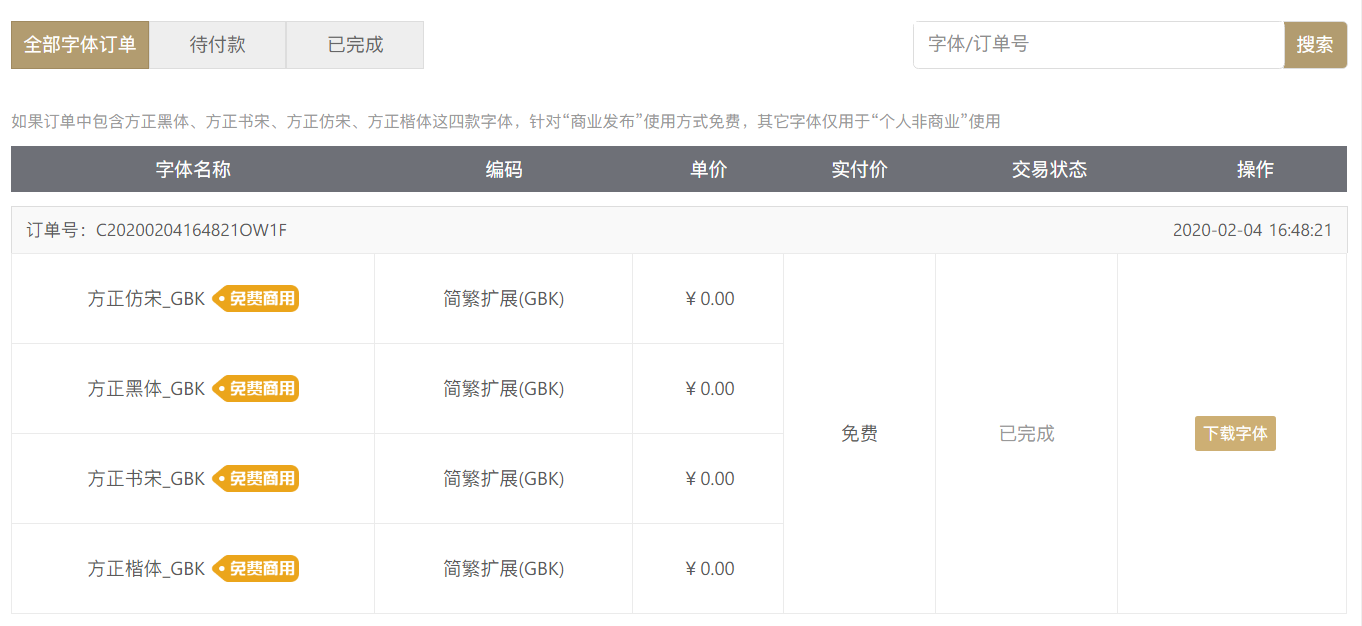
\includegraphics[width=0.9\textwidth]{founder.png}
\end{figure}

\subsubsection{其他中文字体}
如果你想完全自定义字体\footnote{这里仍然以方正字体为例。},你可以选择 \lstinline{chinesefont=nofont},然后在导言区设置
\begin{lstlisting}
\setCJKmainfont[BoldFont={FZHei-B01},ItalicFont={FZKai-Z03}]{FZShuSong-Z01}
\setCJKsansfont[BoldFont={FZHei-B01},ItalicFont={FZHei-B01}]{FZHei-B01}
\setCJKmonofont[BoldFont={FZHei-B01},ItalicFont={FZHei-B01}]{FZFangSong-Z02}
\setCJKfamilyfont{zhsong}{FZShuSong-Z01}
\setCJKfamilyfont{zhhei}{FZHei-B01}
\setCJKfamilyfont{zhkai}{FZKai-Z03}
\setCJKfamilyfont{zhfs}{FZFangSong-Z02}
\newcommand*{\songti}{\CJKfamily{zhsong}}
\newcommand*{\heiti}{\CJKfamily{zhhei}}
\newcommand*{\kaishu}{\CJKfamily{zhkai}}
\newcommand*{\fangsong}{\CJKfamily{zhfs}}
\end{lstlisting}


\subsection[颜色主题]{颜色主题\footnote{测试章节脚注。}}

本模板内置 5 套颜色主题,分别是 \textcolor{eblue}{blue}(默认),\textcolor{egreen}{green}, \textcolor{ecyan}{cyan}, \textcolor{sakura}{sakura} 和 \textcolor{black}{black}。如果不需要颜色,可以选择黑色(black)主题。颜色主题的设置方法:
\begin{lstlisting}[frame=none]
  \documentclass[green]{elegantnote}
  \documentclass[color=green]{elegantnote}
  ...
  \documentclass[black]{elegantnote}
  \documentclass[color=black]{elegantnote}
\end{lstlisting}


\subsection{语言模式}

本模板内含两套语言环境,改变语言环境会改变图表标题的引导词(图,表),文章结构词(比如目录,参考文献等),以及定理环境中的引导词(比如定理,引理等)。不同语言模式的启用如下:
\begin{lstlisting}[frame=none]
  \documentclass[cn]{elegantnote}
  \documentclass[lang=cn]{elegantnote}
  \documentclass[en]{elegantnote}
  \documentclass[lang=en]{elegantnote}
\end{lstlisting}

\begin{note}
只有中文模式才可输入中文,如果需要在英文模式下输入中文,可以自行添加 \lstinline{ctex} 宏包\footnote{需要使用 \lstinline{scheme=plain} 选项才不会把标题改为中文。}或者使用 \lstinline{xeCJK} 宏包设置字体。另外如果在笔记中使用了抄录环境(\lstinline{lstlisting}),并且里面有中文字符,请务必使用 \hologo{XeLaTeX} 编译。
\end{note}


\subsection{定理类环境}

此模板采用了 \lstinline{amsthm} 中的定理样式,使用了 4 类定理样式,所包含的环境分别为
\begin{itemize}
  \item \textbf{定理类}:theorem,lemma,proposition,corollary;
  \item \textbf{定义类}:definition,conjecture,example;
  \item \textbf{备注类}:remark,note,case;
  \item \textbf{证明类}:proof。
\end{itemize}

\begin{remark}
在选用 \lstinline{lang=cn} 时,定理类环境的引导词全部会改为中文。
\end{remark}


\section{写作示例}

我们将通过三个步骤定义可测函数的积分。首先定义非负简单函数的积分。以下设 $E$ 是 $\mathcal{R}^n$ 中的可测集。

\begin{definition}[可积性]
设 $ f(x)=\sum\limits_{i=1}^{k} a_i \chi_{A_i}(x)$ 是 $E$ 上的非负简单函数,其中 $\{A_1,A_2,\ldots$, $A_k\}$ 是 $E$ 上的一个可测分割,$a_1,a_2,\ldots,a_k$ 是非负实数。定义 $f$ 在 $E$ 上的积分为 1. 3
\begin{equation}
   \label{inter}
   \int_{E} f dx = \sum_{i=1}^k a_i m(A_i).
\end{equation}
一般情况下 $0 \leq \int_{E} f dx \leq \infty$。若 $\int_{E} f dx < \infty$,则称 $f$ 在 $E$ 上可积。
\end{definition}

一个自然的问题是,Lebesgue 积分与我们所熟悉的 Riemann 积分有什么联系和区别?之后我们将详细讨论 Riemann 积分与 Lebesgue 积分的关系。这里只看一个简单的例子。设 $D(x)$ 是区间 $[0,1]$ 上的 Dirichlet 函数。即 $D(x)=\chi_{Q_0}(x)$,其中 $Q_0$ 表示 $[0,1]$ 中的有理数的全体。根据非负简单函数积分的定义,$D(x)$ 在 $[0,1]$ 上的 Lebesgue 积分为
\begin{equation}\label{inter2}
  \int_0^1 D(x)dx = \int_0^1 \chi_{Q_0} (x) dx = m(Q_0) = 0
\end{equation}
即 $D(x)$ 在 $[0,1]$ 上是 Lebesgue 可积的并且积分值为零。但 $D(x)$ 在 $[0,1]$ 上不是 Riemann 可积的。

\begin{table}[htbp]
  \centering
  \small
  \caption{燃油效率与汽车价格}
    \begin{tabular}{lcc}
    \toprule
                  &       (1)         &        (2)      \\
    \midrule
    燃油效率      &   -238.90***      &      -49.51     \\
                  &    (53.08)        &      (86.16)    \\
    汽车重量      &                   &        1.75***  \\
                  &                   &       (0.641)   \\
    常数项        &  11253.00***      &    1946.00      \\
                  &  (1171.00)        &   (3597.00)     \\
    观测数        &     74            &      74         \\
    $R^2$         &      0.220        &       0.293     \\
    \bottomrule
    \end{tabular}%
  \label{tab:reg}%
\end{table}%

\begin{theorem}[Fubini 定理]\label{thm:fubi}
若 $f(x,y)$ 是 $\mathcal{R}^p\times\mathcal{R}^q$ 上的非负可测函数,则对几乎处处的 $x\in \mathcal{R}^p$,$f(x,y)$ 作为 $y$ 的函数是 $\mathcal{R}^q$ 上的非负可测函数,$g(x)=\int_{\mathcal{R}^q}f(x,y) dy$ 是 $\mathcal{R}^p$ 上的非负可测函数。并且
\begin{equation}\label{eq:461}
  \int_{\mathcal{R}^p\times\mathcal{R}^q} f(x,y) dxdy=\int_{\mathcal{R}^p}\left(\int_{\mathcal{R}^q}f(x,y)dy\right)dx.
\end{equation}
\end{theorem}

\begin{proof}
Let $z$ be some element of $xH \cap yH$.  Then $z = xa$ for some $a \in H$, and $z = yb$ for some $b \in H$. If $h$ is any element of $H$ then $ah \in H$ and $a^{-1}h \in H$, since $H$ is a subgroup of $G$. But $zh = x(ah)$ and $xh = z(a^{-1}h)$ for all $h \in H$. Therefore $zH \subset xH$ and $xH \subset zH$, and thus $xH = zH$.  Similarly $yH = zH$, and thus $xH = yH$, as required.
\end{proof}


回归分析(regression analysis) 是确定两种或两种以上变量间相互依赖的定量关系的一种统计分析方法。根据定理~\ref{thm:fubi},其运用十分广泛,回归分析按照涉及的变量的多少,分为一元回归和多元回归分析;按照因变量的多少,可分为简单回归分析和多重回归分析;按照自变量和因变量之间的关系类型,可分为线性回归分析和非线性回归分析。


\section{协作人员招募}

招募 Elegant\LaTeX{} 的协作人员,没有工资。工作内容:翻译 Elegant\LaTeX{} 系列模板相关的文稿(中翻英),维护模板的 wiki(主要涉及 Markdown),如果有公众号文稿写作经历的话,也可以帮忙写微信稿。本公告长期有效。

目前 ElegantLaTeX 共有 4 名协作人员,分别是
\begin{itemize}
  \item 官方文档翻译: \href{https://github.com/peggy2006xzyz}{YPY};
  \item GitHub 维基维护: \href{https://github.com/izinngo}{Ingo Zinngo}、\href{https://github.com/xiaohao890809}{追寻原风景};
  \item QQ 群管理员: \href{https://github.com/sikouhjw}{Sikouhjw}.
\end{itemize}

在此感谢他们无私的奉献!


\section{致谢}

截止到 2020 年 04 月 12 日,ElegantNote 2.30 版本发布,ElegantNote 模板在 GitHub 上的收藏数(star)达到了 263。在此特别感谢 China\TeX{} 以及 \href{http://www.latexstudio.net/}{\LaTeX{} 工作室}对于本系列模板的大力宣传与推广。如果你喜欢我们的模板,你可以在 GitHub 上收藏(Star)我们的模板。

\begin{figure}[htbp]
  \centering
  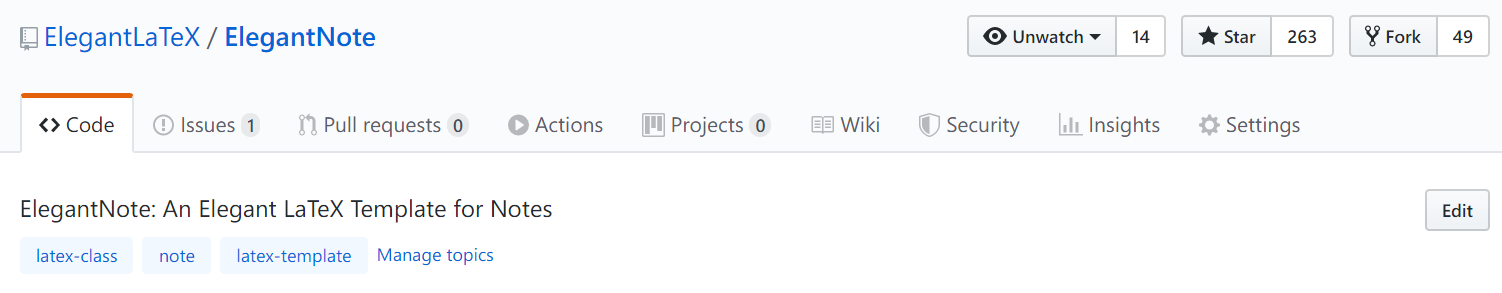
\includegraphics[width=\textwidth]{star.png}
  \caption{一键三连求赞}
\end{figure}


\section{捐赠}

如果您非常喜爱我们的模板,你还可以选择捐赠以表达您对我们模板和我的支持!

\begin{figure}[htbp]
  \centering
  
\includegraphics[width=0.4\textwidth]{donate.jpg}
\end{figure}

\textbf{赞赏费用的使用解释权归 Elegant\LaTeX{} 所有,并且不接受监督,请自愿理性打赏}。10 元以上的赞赏,我们将列入捐赠榜,并且发放捐赠纪念证(全部),谢谢各位金主!

\begin{table}[htbp]
  \scriptsize
  \centering
  \caption{Elegant\LaTeX{} 系列模板捐赠榜}
    \begin{tabular}{*{8}{>{\scriptsize}c}}
    \toprule
    \textbf{捐赠者} & \textbf{金额} & \textbf{时间} & \textbf{渠道} & \textbf{捐赠者} & \textbf{金额} & \textbf{时间} & \textbf{渠道} \\
    \midrule
    Lerh  & 10 RMB & 2019/05/15 & 微信    & 越过地平线 & 10 RMB & 2019/05/15 & 微信 \\
    银桑    & 20 RMB & 2019/05/27 & 微信    & *空    & 10 RMB & 2019/05/30 & 微信 \\
    latexstudio.net & 666 RMB & 2019/06/05 & 支付宝   & A*n   & 40 RMB & 2019/06/15 & 微信 \\
    * 夏   & 22 RMB & 2019/06/15 & 微信    & * 倩   & 21 RMB  & 2019/06/15 & 微信 \\
    Cassis & 11 RMB & 2019/06/30 & 微信    & *君    & 10 RMB & 2019/07/23 & 微信 \\
    P*u   & 50 RMB & 2019/07/30 & 微信    & *萌    & 19 RMB & 2019/08/28 & 微信 \\
    曲豆豆   & 10 RMB & 2019/08/28 & 微信    & 李博    & 100 RMB & 2019/10/06 & 微信 \\
    Njustsll & 10 RMB & 2019/10/11 & 微信    & 刘志阔   & 99.99 RMB & 2019/10/15 & 支付宝 \\
    * 韬   & 16 RMB & 2019/10/17 & 微信    & 赤霓    & 12 RMB & 2019/10/17 & 支付宝 \\
    追寻原风景 & 10 RMB & 2019/10/28 & 微信    & 郭德良   & 88 RMB & 2019/11/03 & 微信 \\
    自强不息  & 20 RMB & 2019/11/04 & 支付宝   & 读书之虫  & 20 RMB & 2019/11/18 & 微信 \\
    *等    & 10 RMB & 2019/11/18 & 微信    & *哲    & 20 RMB & 2019/11/18 & 微信 \\
    佚名    & 10 RMB & 2019/11/24 & 微信    & Jiye Qian & 66 RMB & 2019/12/04 & 微信 \\
    * 阳   & 20 RMB & 2019/12/05 & 微信    & Catcher & 11 RMB & 2019/12/08 & 支付宝 \\
    希尔波特门徒 & 10 RMB & 2019/12/09 & 支付宝   & * 伟   & 10 RMB & 2019/12/09 & 微信 \\
    Simon & 20 RMB & 2019/12/11 & 支付宝   & 流殇丶浅忆 & 66.60 RMB & 2019/12/18 & 支付宝 \\
    羽     & 10 RMB & 2019/12/20 & 支付宝   & * 琛   & 15 RMB & 2019/12/20 & 微信 \\
    随风    & 20 RMB & 2019/12/27 & 支付宝   & Ws    & 23.30 RMB & 2019/12/28 & 微信 \\
    初八    & 100 RMB  & 2020/01/02 & 支付宝   & p*e   & 20 RMB & 2020/01/03 & 微信 \\
    Shunmx & 100 RMB & 2020/01/03 & 微信    & hj    & 10 RMB & 2020/01/03 & 微信 \\
    F*5   & 10 RMB & 2020/01/03 & 微信    & S*m   & 20.20 RMB & 2020/01/03 & 微信 \\
    二代青雉  & 13 RMB & 2020/01/14 & 支付宝   & *?    & 66 RMB & 2020/01/15 & 微信 \\
    Mr. Xiong & 20 RMB & 2020/01/17 & 微信    & *博    & 15 RMB & 2020/01/18 & 微信 \\
    * 者  & 10 RMB & 2020/02/02 & 微信    & Jackie  &  88.80 RMB  &  2020/02/09 & 微信 \\
    Henry\_Sun、 & 50 RMB & 2020/02/14 & 支付宝 & * 桥  & 50 RMB & 2020/02/21 & 微信 \\
    昀琏 & 10 RMB & 2020/03/02 & 支付宝 & S*y  &  10 RMB  &  2020/03/15 & 微信 \\
    * 哥  & 66.66 RMB & 2020/03/17 & 微信    &   K*e & 30 RMB & 2020/03/30 & 微信\\
    * 阳  &  20 RMB  &  2020/04/02 & 微信 & 士*n  & 30 RMB & 2020/04/11 & 微信 \\
    \bottomrule
    \end{tabular}%
  \label{tab:donation}%
\end{table}%


\section{常见问题 FAQ}

\begin{enumerate}[label=\arabic*).]
  \item \textit{如何删除版本信息?}\\
    导言区不写 \lstinline|\version{x.xx}| 即可。
  \item \textit{如何删除日期?}\\
    与版本 \lstinline{\version} 不同的是,导言区不写或注释 \lstinline{\date} 的话,仍然会打印出当日日期,原因是 \lstinline{\date} 有默认参数。如果不需要日期的话,日期可以留空即可,也即 \lstinline|\date{}|。
  \item \textit{如何获得中文日期?}\\
    为了获得中文日期,必须在中文模式下,使用 \lstinline|\date{\zhdate{2019/12/09}}|,如果需要当天的汉化日期,可以使用 \lstinline|\date{\zhtoday}|,这两个命令都来源于 \href{https://ctan.org/pkg/zhnumber}{\lstinline{zhnumber}} 宏包。
  \item \textit{如何添加多个作者?}\\
    在 \lstinline{\author} 里面使用 \lstinline{\and},作者单位可以用 \lstinline{\\} 换行。
    \begin{lstlisting}
      \author{author 1\\ org. 1 \and author 2 \\ org. 2 }
    \end{lstlisting}
\end{enumerate}

\fi

\end{document}
